% ferryGL white paper. Build with `make` (latexmk and pdfLaTeX); see README.md.
\documentclass[11pt,a4paper]{article}

\usepackage[a4paper, top=2.5cm, bottom=2.7cm, left=2.5cm, right=2.5cm, headheight=14pt]{geometry}
\usepackage[T1]{fontenc}
\usepackage[utf8]{inputenc}
\usepackage{csquotes}
\usepackage{libertinus}
\usepackage[varqu, scaled=0.95]{zi4}
\usepackage[final]{microtype}
\usepackage{xcolor}
\usepackage{graphicx}
\usepackage{amsmath}
\usepackage{booktabs}
\usepackage{tabularx}
\usepackage{array}
\usepackage[shortlabels]{enumitem}
\usepackage[font=small, labelfont=bf, labelsep=period, skip=6pt]{caption}
\usepackage[group-separator={,}, group-minimum-digits=4]{siunitx}
\usepackage{algorithm}
\usepackage[noend]{algpseudocode}
\usepackage{listings}
\usepackage{fancyhdr}
\usepackage{tikz}
\usetikzlibrary{arrows.meta, positioning, calc, shapes.geometric, fit, backgrounds, patterns}
\usepackage{pgfplots}
\pgfplotsset{compat=1.18}
\usepgfplotslibrary{groupplots}
\usepackage{pgfplotstable}
\usepackage[numbers, sort&compress]{natbib}
\usepackage[hidelinks, pdfusetitle]{hyperref}
\usepackage[capitalize, nameinlink, noabbrev]{cleveref}

\graphicspath{{../../assets/}}
% Colors and TikZ styles shared by the figures. The colors are the website's
% (site/style.css), so the figures match ferryGL's documentation.
\definecolor{fgNavy}{HTML}{0C2137}
\definecolor{fgTeal}{HTML}{0A7C6C}
\definecolor{fgBrand}{HTML}{24D5BB}
\definecolor{fgBlue}{HTML}{0B6AA6}
\definecolor{fgMuted}{HTML}{45566B}
\definecolor{fgSubtle}{HTML}{66778C}
\definecolor{fgBorder}{HTML}{CDD7E2}
\definecolor{fgSoft}{HTML}{F5F8FB}
\definecolor{fgCode}{HTML}{F2F5F9}
\definecolor{fgRed}{HTML}{C2185B}
\definecolor{stTodo}{HTML}{8592A3}
\definecolor{stProgress}{HTML}{E2A336}
\definecolor{stReview}{HTML}{1FA37A}
\definecolor{stDone}{HTML}{4F72E8}
\definecolor{stCanceled}{HTML}{8592A3}

\tikzset{
  >={Stealth[length=2.2mm]},
  every node/.style={font=\sffamily\small, text=fgNavy},
  box/.style={draw=fgBorder, fill=white, rounded corners=2pt, line width=0.6pt,
    inner sep=4pt, align=center},
  region/.style={draw=fgBorder, fill=fgSoft, rounded corners=4pt, line width=0.6pt},
  stage/.style={draw=fgNavy, fill=white, rounded corners=2pt, line width=0.7pt,
    minimum height=8mm, minimum width=15mm, align=center},
  store/.style={cylinder, shape border rotate=90, aspect=0.18, draw=fgNavy, fill=fgSoft,
    line width=0.7pt, minimum width=24mm, minimum height=11mm, align=center},
  flow/.style={->, line width=0.8pt, draw=fgNavy},
  readflow/.style={->, line width=0.8pt, draw=fgBlue},
  writeflow/.style={->, line width=0.8pt, draw=fgTeal},
  note/.style={font=\sffamily\scriptsize, text=fgMuted, align=center},
  statekey/.style={font=\ttfamily\scriptsize, text=fgNavy},
  status/.style={rounded corners=2pt, text=white, font=\sffamily\scriptsize\bfseries,
    minimum height=4.6mm, minimum width=19mm, inner sep=2pt},
  todo/.style={status, fill=stTodo},
  progress/.style={status, fill=stProgress},
  review/.style={status, fill=stReview},
  done/.style={status, fill=stDone},
  canceled/.style={status, fill=stCanceled, pattern color=white},
}

\pgfplotsset{
  ferrygl/.style={
    label style={font=\sffamily\small},
    tick label style={font=\sffamily\scriptsize},
    /pgf/number format/assume math mode=true,
    every axis plot/.append style={line width=1.1pt, mark size=1.5pt},
    legend cell align=left,
    legend style={draw=none, fill=none, nodes={font=\sffamily\scriptsize, text=fgNavy}},
    axis line style={fgMuted}, tick style={fgMuted},
  },
}

% Generated by evaluation/simulate.py from the same run as simulation.json.
\newcommand{\SimScenarios}{\num{2000}}
\newcommand{\SimSteps}{\num{12}}
\newcommand{\SimFaultRate}{5\,\%}
\newcommand{\SimSeed}{20261019}
\newcommand{\SimRuns}{\num{74139}}
\newcommand{\SimWrites}{\num{49178}}
\newcommand{\SimEvents}{\num{55538}}
\newcommand{\SimChecks}{\num{427136}}
\newcommand{\SimSafetyChecks}{\num{413071}}
\newcommand{\SimFaultsInjected}{\num{2250}}
\newcommand{\SimRunsWithFailedWrites}{\num{2139}}
\newcommand{\SimOrphans}{\num{776}}
\newcommand{\SimOrphansAdopted}{\num{776}}
\newcommand{\SimMultiRiderObservations}{\num{846}}
\newcommand{\SimActionCreate}{\num{11421}}
\newcommand{\SimActionUpdate}{\num{5734}}
\newcommand{\SimActionLink}{\num{1598}}
\newcommand{\SimActionRecord}{\num{821}}
\newcommand{\SimActionAdopt}{\num{412}}
\newcommand{\SimActionSkip}{\num{133}}
\newcommand{\SimChecksDryRun}{\num{24000}}
\newcommand{\SimViolationsDryRun}{\num{0}}
\newcommand{\SimChecksQuiescent}{\num{24000}}
\newcommand{\SimViolationsQuiescent}{\num{0}}
\newcommand{\SimChecksOneHome}{\num{80923}}
\newcommand{\SimViolationsOneHome}{\num{0}}
\newcommand{\SimChecksOwnership}{\num{49178}}
\newcommand{\SimViolationsOwnership}{\num{0}}
\newcommand{\SimChecksStatusSource}{\num{4742}}
\newcommand{\SimViolationsStatusSource}{\num{0}}
\newcommand{\SimChecksEditsWin}{\num{4098}}
\newcommand{\SimViolationsEditsWin}{\num{0}}
\newcommand{\SimChecksCoverage}{\num{86168}}
\newcommand{\SimViolationsCoverage}{\num{0}}
\newcommand{\SimChecksConsistent}{\num{75204}}
\newcommand{\SimViolationsConsistent}{\num{0}}
\newcommand{\SimChecksForeignMetadata}{\num{11302}}
\newcommand{\SimViolationsForeignMetadata}{\num{0}}
\newcommand{\SimChecksMinimalData}{\num{49178}}
\newcommand{\SimViolationsMinimalData}{\num{0}}
\newcommand{\SimChecksRecovery}{\num{4278}}
\newcommand{\SimViolationsRecovery}{\num{0}}
\newcommand{\SimChecksOrderIndependent}{\num{14065}}
\newcommand{\SimViolationsOrderIndependent}{\num{29}}

% Generated by evaluation/agent_cost.py.
\newcommand{\AgentRuns}{\num{48000}}
\newcommand{\TokLeanPayload}{2.93}
\newcommand{\TokLeanText}{4.06}
\newcommand{\TokLeanPrinted}{3.70}
\newcommand{\TokPlausiblePayload}{2.81}
\newcommand{\TokPlausibleText}{4.02}
\newcommand{\TokPlausiblePrinted}{3.66}
\newcommand{\AgentItemsMedian}{\num{3}}
\newcommand{\AgentCallsMedian}{\num{12}}
\newcommand{\AgentFixedLean}{\num{3361}}
\newcommand{\AgentFixedPlausible}{\num{3391}}
\newcommand{\AgentFixedLeanDelegating}{\num{735}}
\newcommand{\AgentFixedPlausibleDelegating}{\num{736}}
\newcommand{\HistLeanHaikuTokens}{\num{15302}}
\newcommand{\HistLeanHaikuDollars}{\$0.0013}
\newcommand{\HistLeanHaikuQuiet}{46\,\%}
\newcommand{\HistLeanSonnetTokens}{\num{15302}}
\newcommand{\HistLeanSonnetDollars}{\$0.025}
\newcommand{\HistLeanSonnetQuiet}{46\,\%}
\newcommand{\HistLeanOpusTokens}{\num{15302}}
\newcommand{\HistLeanOpusDollars}{\$0.051}
\newcommand{\HistLeanOpusQuiet}{46\,\%}
\newcommand{\HistPlausibleHaikuTokens}{\num{29583}}
\newcommand{\HistPlausibleHaikuDollars}{\$0.0027}
\newcommand{\HistPlausibleHaikuQuiet}{46\,\%}
\newcommand{\HistPlausibleSonnetTokens}{\num{29583}}
\newcommand{\HistPlausibleSonnetDollars}{\$0.052}
\newcommand{\HistPlausibleSonnetQuiet}{46\,\%}
\newcommand{\HistPlausibleOpusTokens}{\num{29583}}
\newcommand{\HistPlausibleOpusDollars}{\$0.10}
\newcommand{\HistPlausibleOpusQuiet}{46\,\%}
\newcommand{\HistLeanDelegatingHaikuTokens}{\num{3143}}
\newcommand{\HistLeanDelegatingHaikuDollars}{\$0.00039}
\newcommand{\HistLeanDelegatingHaikuQuiet}{49\,\%}
\newcommand{\HistLeanDelegatingSonnetTokens}{\num{3143}}
\newcommand{\HistLeanDelegatingSonnetDollars}{\$0.0077}
\newcommand{\HistLeanDelegatingSonnetQuiet}{49\,\%}
\newcommand{\HistLeanDelegatingOpusTokens}{\num{3143}}
\newcommand{\HistLeanDelegatingOpusDollars}{\$0.015}
\newcommand{\HistLeanDelegatingOpusQuiet}{49\,\%}
\newcommand{\HistPlausibleDelegatingHaikuTokens}{\num{5545}}
\newcommand{\HistPlausibleDelegatingHaikuDollars}{\$0.0011}
\newcommand{\HistPlausibleDelegatingHaikuQuiet}{50\,\%}
\newcommand{\HistPlausibleDelegatingSonnetTokens}{\num{5545}}
\newcommand{\HistPlausibleDelegatingSonnetDollars}{\$0.022}
\newcommand{\HistPlausibleDelegatingSonnetQuiet}{50\,\%}
\newcommand{\HistPlausibleDelegatingOpusTokens}{\num{5545}}
\newcommand{\HistPlausibleDelegatingOpusDollars}{\$0.044}
\newcommand{\HistPlausibleDelegatingOpusQuiet}{50\,\%}
\newcommand{\DelegationLeanRatioTen}{8}
\newcommand{\DelegationLeanSavesTen}{4}
\newcommand{\DelegationPlausibleRatioTen}{7}
\newcommand{\DelegationPlausibleSavesTen}{3}
\newcommand{\DelegationLeanRatioHundred}{27}
\newcommand{\DelegationLeanSavesHundred}{15}
\newcommand{\DelegationPlausibleRatioHundred}{38}
\newcommand{\DelegationPlausibleSavesHundred}{9}
\newcommand{\DelegationLeanRatioEightHundred}{122}
\newcommand{\DelegationLeanSavesEightHundred}{79}
\newcommand{\DelegationPlausibleRatioEightHundred}{934}
\newcommand{\DelegationPlausibleSavesEightHundred}{77}
\newcommand{\DelegationRatioTenLow}{7}
\newcommand{\DelegationRatioTenHigh}{8}
\newcommand{\DelegationSavesTenLow}{3}
\newcommand{\DelegationSavesTenHigh}{4}
\newcommand{\DelegationRatioHundredLow}{27}
\newcommand{\DelegationRatioHundredHigh}{38}
\newcommand{\DelegationSavesHundredLow}{9}
\newcommand{\DelegationSavesHundredHigh}{15}
\newcommand{\DelegationRatioEightHundredLow}{122}
\newcommand{\DelegationRatioEightHundredHigh}{934}
\newcommand{\DelegationSavesEightHundredLow}{77}
\newcommand{\DelegationSavesEightHundredHigh}{79}
\newcommand{\RunLeanHaikuTwentyFive}{\$0.0025}
\newcommand{\TokLeanHaikuTwentyFive}{\num{35551}}
\newcommand{\MonthLeanHaikuTwentyFive}{\$0.11}
\newcommand{\HourlyLeanHaikuTwentyFive}{\$0.43}
\newcommand{\RunLeanSonnetTwentyFive}{\$0.047}
\newcommand{\TokLeanSonnetTwentyFive}{\num{35551}}
\newcommand{\MonthLeanSonnetTwentyFive}{\$2.08}
\newcommand{\HourlyLeanSonnetTwentyFive}{\$8.31}
\newcommand{\RunLeanOpusTwentyFive}{\$0.094}
\newcommand{\TokLeanOpusTwentyFive}{\num{35551}}
\newcommand{\MonthLeanOpusTwentyFive}{\$4.15}
\newcommand{\HourlyLeanOpusTwentyFive}{\$16.62}
\newcommand{\RunPlausibleHaikuTwentyFive}{\$0.0044}
\newcommand{\TokPlausibleHaikuTwentyFive}{\num{58691}}
\newcommand{\MonthPlausibleHaikuTwentyFive}{\$0.19}
\newcommand{\HourlyPlausibleHaikuTwentyFive}{\$0.77}
\newcommand{\RunPlausibleSonnetTwentyFive}{\$0.084}
\newcommand{\TokPlausibleSonnetTwentyFive}{\num{58691}}
\newcommand{\MonthPlausibleSonnetTwentyFive}{\$3.69}
\newcommand{\HourlyPlausibleSonnetTwentyFive}{\$14.77}
\newcommand{\RunPlausibleOpusTwentyFive}{\$0.17}
\newcommand{\TokPlausibleOpusTwentyFive}{\num{58691}}
\newcommand{\MonthPlausibleOpusTwentyFive}{\$7.39}
\newcommand{\HourlyPlausibleOpusTwentyFive}{\$29.54}
\newcommand{\RunLeanDelegatingHaikuTwentyFive}{\$0.00040}
\newcommand{\TokLeanDelegatingHaikuTwentyFive}{\num{3202}}
\newcommand{\MonthLeanDelegatingHaikuTwentyFive}{\$0.018}
\newcommand{\HourlyLeanDelegatingHaikuTwentyFive}{\$0.070}
\newcommand{\RunLeanDelegatingSonnetTwentyFive}{\$0.0078}
\newcommand{\TokLeanDelegatingSonnetTwentyFive}{\num{3202}}
\newcommand{\MonthLeanDelegatingSonnetTwentyFive}{\$0.34}
\newcommand{\HourlyLeanDelegatingSonnetTwentyFive}{\$1.37}
\newcommand{\RunLeanDelegatingOpusTwentyFive}{\$0.016}
\newcommand{\TokLeanDelegatingOpusTwentyFive}{\num{3202}}
\newcommand{\MonthLeanDelegatingOpusTwentyFive}{\$0.69}
\newcommand{\HourlyLeanDelegatingOpusTwentyFive}{\$2.75}
\newcommand{\RunPlausibleDelegatingHaikuTwentyFive}{\$0.0011}
\newcommand{\TokPlausibleDelegatingHaikuTwentyFive}{\num{5605}}
\newcommand{\MonthPlausibleDelegatingHaikuTwentyFive}{\$0.048}
\newcommand{\HourlyPlausibleDelegatingHaikuTwentyFive}{\$0.19}
\newcommand{\RunPlausibleDelegatingSonnetTwentyFive}{\$0.022}
\newcommand{\TokPlausibleDelegatingSonnetTwentyFive}{\num{5605}}
\newcommand{\MonthPlausibleDelegatingSonnetTwentyFive}{\$0.96}
\newcommand{\HourlyPlausibleDelegatingSonnetTwentyFive}{\$3.85}
\newcommand{\RunPlausibleDelegatingOpusTwentyFive}{\$0.044}
\newcommand{\TokPlausibleDelegatingOpusTwentyFive}{\num{5605}}
\newcommand{\MonthPlausibleDelegatingOpusTwentyFive}{\$1.92}
\newcommand{\HourlyPlausibleDelegatingOpusTwentyFive}{\$7.69}
\newcommand{\FirstRunLeanHaikuHundred}{\$0.017}
\newcommand{\FirstTokLeanHaikuHundred}{\num{102343}}
\newcommand{\FirstRunLeanSonnetHundred}{\$0.35}
\newcommand{\FirstTokLeanSonnetHundred}{\num{102343}}
\newcommand{\FirstRunLeanOpusHundred}{\$0.69}
\newcommand{\FirstTokLeanOpusHundred}{\num{102343}}
\newcommand{\FirstRunPlausibleHaikuHundred}{\$0.053}
\newcommand{\FirstTokPlausibleHaikuHundred}{\num{2234995}}
\newcommand{\FirstRunPlausibleSonnetHundred}{\$0.85}
\newcommand{\FirstTokPlausibleSonnetHundred}{\num{2234995}}
\newcommand{\FirstRunPlausibleOpusHundred}{\$1.70}
\newcommand{\FirstTokPlausibleOpusHundred}{\num{2234995}}
\newcommand{\FirstRunLeanDelegatingHaikuHundred}{\$0.00099}
\newcommand{\FirstTokLeanDelegatingHaikuHundred}{\num{10059}}
\newcommand{\FirstRunLeanDelegatingSonnetHundred}{\$0.019}
\newcommand{\FirstTokLeanDelegatingSonnetHundred}{\num{10059}}
\newcommand{\FirstRunLeanDelegatingOpusHundred}{\$0.039}
\newcommand{\FirstTokLeanDelegatingOpusHundred}{\num{10059}}
\newcommand{\FirstRunPlausibleDelegatingHaikuHundred}{\$0.0017}
\newcommand{\FirstTokPlausibleDelegatingHaikuHundred}{\num{12537}}
\newcommand{\FirstRunPlausibleDelegatingSonnetHundred}{\$0.034}
\newcommand{\FirstTokPlausibleDelegatingSonnetHundred}{\num{12537}}
\newcommand{\FirstRunPlausibleDelegatingOpusHundred}{\$0.067}
\newcommand{\FirstTokPlausibleDelegatingOpusHundred}{\num{12537}}
\newcommand{\RunLeanHaikuHundred}{\$0.0065}
\newcommand{\TokLeanHaikuHundred}{\num{91620}}
\newcommand{\MonthLeanHaikuHundred}{\$0.28}
\newcommand{\HourlyLeanHaikuHundred}{\$1.14}
\newcommand{\RunLeanSonnetHundred}{\$0.12}
\newcommand{\TokLeanSonnetHundred}{\num{91620}}
\newcommand{\MonthLeanSonnetHundred}{\$5.46}
\newcommand{\HourlyLeanSonnetHundred}{\$21.82}
\newcommand{\PeakLeanHundred}{\num{35955}}
\newcommand{\RunLeanOpusHundred}{\$0.25}
\newcommand{\TokLeanOpusHundred}{\num{91620}}
\newcommand{\MonthLeanOpusHundred}{\$10.91}
\newcommand{\HourlyLeanOpusHundred}{\$43.64}
\newcommand{\RunPlausibleHaikuHundred}{\$0.011}
\newcommand{\TokPlausibleHaikuHundred}{\num{217857}}
\newcommand{\MonthPlausibleHaikuHundred}{\$0.50}
\newcommand{\HourlyPlausibleHaikuHundred}{\$1.99}
\newcommand{\RunPlausibleSonnetHundred}{\$0.21}
\newcommand{\TokPlausibleSonnetHundred}{\num{217857}}
\newcommand{\MonthPlausibleSonnetHundred}{\$9.24}
\newcommand{\HourlyPlausibleSonnetHundred}{\$36.96}
\newcommand{\PeakPlausibleHundred}{\num{55454}}
\newcommand{\RunPlausibleOpusHundred}{\$0.42}
\newcommand{\TokPlausibleOpusHundred}{\num{217857}}
\newcommand{\MonthPlausibleOpusHundred}{\$18.48}
\newcommand{\HourlyPlausibleOpusHundred}{\$73.91}
\newcommand{\RunLeanDelegatingHaikuHundred}{\$0.00041}
\newcommand{\TokLeanDelegatingHaikuHundred}{\num{3364}}
\newcommand{\MonthLeanDelegatingHaikuHundred}{\$0.018}
\newcommand{\HourlyLeanDelegatingHaikuHundred}{\$0.072}
\newcommand{\RunLeanDelegatingSonnetHundred}{\$0.0081}
\newcommand{\TokLeanDelegatingSonnetHundred}{\num{3364}}
\newcommand{\MonthLeanDelegatingSonnetHundred}{\$0.36}
\newcommand{\HourlyLeanDelegatingSonnetHundred}{\$1.42}
\newcommand{\PeakLeanDelegatingHundred}{\num{1177}}
\newcommand{\RunLeanDelegatingOpusHundred}{\$0.016}
\newcommand{\TokLeanDelegatingOpusHundred}{\num{3364}}
\newcommand{\MonthLeanDelegatingOpusHundred}{\$0.71}
\newcommand{\HourlyLeanDelegatingOpusHundred}{\$2.85}
\newcommand{\RunPlausibleDelegatingHaikuHundred}{\$0.0011}
\newcommand{\TokPlausibleDelegatingHaikuHundred}{\num{5769}}
\newcommand{\MonthPlausibleDelegatingHaikuHundred}{\$0.049}
\newcommand{\HourlyPlausibleDelegatingHaikuHundred}{\$0.20}
\newcommand{\RunPlausibleDelegatingSonnetHundred}{\$0.022}
\newcommand{\TokPlausibleDelegatingSonnetHundred}{\num{5769}}
\newcommand{\MonthPlausibleDelegatingSonnetHundred}{\$0.97}
\newcommand{\HourlyPlausibleDelegatingSonnetHundred}{\$3.90}
\newcommand{\PeakPlausibleDelegatingHundred}{\num{1979}}
\newcommand{\RunPlausibleDelegatingOpusHundred}{\$0.044}
\newcommand{\TokPlausibleDelegatingOpusHundred}{\num{5769}}
\newcommand{\MonthPlausibleDelegatingOpusHundred}{\$1.95}
\newcommand{\HourlyPlausibleDelegatingOpusHundred}{\$7.79}
\newcommand{\QuietRunLeanHaikuHundred}{\$0.0056}
\newcommand{\QuietTokLeanHaikuHundred}{\num{54966}}
\newcommand{\QuietRunLeanSonnetHundred}{\$0.11}
\newcommand{\QuietTokLeanSonnetHundred}{\num{54966}}
\newcommand{\QuietRunLeanOpusHundred}{\$0.22}
\newcommand{\QuietTokLeanOpusHundred}{\num{54966}}
\newcommand{\QuietRunPlausibleHaikuHundred}{\$0.0092}
\newcommand{\QuietTokPlausibleHaikuHundred}{\num{106048}}
\newcommand{\QuietRunPlausibleSonnetHundred}{\$0.18}
\newcommand{\QuietTokPlausibleSonnetHundred}{\num{106048}}
\newcommand{\QuietRunPlausibleOpusHundred}{\$0.36}
\newcommand{\QuietTokPlausibleOpusHundred}{\num{106048}}
\newcommand{\QuietRunLeanDelegatingHaikuHundred}{\$0.00039}
\newcommand{\QuietTokLeanDelegatingHaikuHundred}{\num{3143}}
\newcommand{\QuietRunLeanDelegatingSonnetHundred}{\$0.0077}
\newcommand{\QuietTokLeanDelegatingSonnetHundred}{\num{3143}}
\newcommand{\QuietRunLeanDelegatingOpusHundred}{\$0.015}
\newcommand{\QuietTokLeanDelegatingOpusHundred}{\num{3143}}
\newcommand{\QuietRunPlausibleDelegatingHaikuHundred}{\$0.0011}
\newcommand{\QuietTokPlausibleDelegatingHaikuHundred}{\num{5546}}
\newcommand{\QuietRunPlausibleDelegatingSonnetHundred}{\$0.022}
\newcommand{\QuietTokPlausibleDelegatingSonnetHundred}{\num{5546}}
\newcommand{\QuietRunPlausibleDelegatingOpusHundred}{\$0.044}
\newcommand{\QuietTokPlausibleDelegatingOpusHundred}{\num{5546}}
\newcommand{\RunLeanHaikuFourHundred}{\$0.080}
\newcommand{\TokLeanHaikuFourHundred}{\num{313151}}
\newcommand{\MonthLeanHaikuFourHundred}{\$3.52}
\newcommand{\HourlyLeanHaikuFourHundred}{\$14.08}
\newcommand{\RunLeanSonnetFourHundred}{\$0.44}
\newcommand{\TokLeanSonnetFourHundred}{\num{313151}}
\newcommand{\MonthLeanSonnetFourHundred}{\$19.27}
\newcommand{\HourlyLeanSonnetFourHundred}{\$77.07}
\newcommand{\RunLeanOpusFourHundred}{\$0.88}
\newcommand{\TokLeanOpusFourHundred}{\num{313151}}
\newcommand{\MonthLeanOpusFourHundred}{\$38.54}
\newcommand{\HourlyLeanOpusFourHundred}{\$154}
\newcommand{\RunPlausibleHaikuFourHundred}{\$0.23}
\newcommand{\TokPlausibleHaikuFourHundred}{\num{1941133}}
\newcommand{\MonthPlausibleHaikuFourHundred}{\$10.06}
\newcommand{\HourlyPlausibleHaikuFourHundred}{\$40.22}
\newcommand{\RunPlausibleSonnetFourHundred}{\$0.83}
\newcommand{\TokPlausibleSonnetFourHundred}{\num{1941133}}
\newcommand{\MonthPlausibleSonnetFourHundred}{\$36.50}
\newcommand{\HourlyPlausibleSonnetFourHundred}{\$146}
\newcommand{\RunPlausibleOpusFourHundred}{\$1.66}
\newcommand{\TokPlausibleOpusFourHundred}{\num{1941133}}
\newcommand{\MonthPlausibleOpusFourHundred}{\$73.01}
\newcommand{\HourlyPlausibleOpusFourHundred}{\$292}
\newcommand{\RunLeanDelegatingHaikuFourHundred}{\$0.00047}
\newcommand{\TokLeanDelegatingHaikuFourHundred}{\num{4061}}
\newcommand{\MonthLeanDelegatingHaikuFourHundred}{\$0.021}
\newcommand{\HourlyLeanDelegatingHaikuFourHundred}{\$0.083}
\newcommand{\RunLeanDelegatingSonnetFourHundred}{\$0.0093}
\newcommand{\TokLeanDelegatingSonnetFourHundred}{\num{4061}}
\newcommand{\MonthLeanDelegatingSonnetFourHundred}{\$0.41}
\newcommand{\HourlyLeanDelegatingSonnetFourHundred}{\$1.63}
\newcommand{\RunLeanDelegatingOpusFourHundred}{\$0.019}
\newcommand{\TokLeanDelegatingOpusFourHundred}{\num{4061}}
\newcommand{\MonthLeanDelegatingOpusFourHundred}{\$0.82}
\newcommand{\HourlyLeanDelegatingOpusFourHundred}{\$3.26}
\newcommand{\RunPlausibleDelegatingHaikuFourHundred}{\$0.0012}
\newcommand{\TokPlausibleDelegatingHaikuFourHundred}{\num{6474}}
\newcommand{\MonthPlausibleDelegatingHaikuFourHundred}{\$0.052}
\newcommand{\HourlyPlausibleDelegatingHaikuFourHundred}{\$0.21}
\newcommand{\RunPlausibleDelegatingSonnetFourHundred}{\$0.023}
\newcommand{\TokPlausibleDelegatingSonnetFourHundred}{\num{6474}}
\newcommand{\MonthPlausibleDelegatingSonnetFourHundred}{\$1.03}
\newcommand{\HourlyPlausibleDelegatingSonnetFourHundred}{\$4.11}
\newcommand{\RunPlausibleDelegatingOpusFourHundred}{\$0.047}
\newcommand{\TokPlausibleDelegatingOpusFourHundred}{\num{6474}}
\newcommand{\MonthPlausibleDelegatingOpusFourHundred}{\$2.05}
\newcommand{\HourlyPlausibleDelegatingOpusFourHundred}{\$8.21}
\newcommand{\RunLeanHaikuEightHundred}{\$0.16}
\newcommand{\TokLeanHaikuEightHundred}{\num{610519}}
\newcommand{\MonthLeanHaikuEightHundred}{\$6.98}
\newcommand{\HourlyLeanHaikuEightHundred}{\$27.92}
\newcommand{\RunLeanSonnetEightHundred}{\$0.86}
\newcommand{\TokLeanSonnetEightHundred}{\num{610519}}
\newcommand{\MonthLeanSonnetEightHundred}{\$37.76}
\newcommand{\HourlyLeanSonnetEightHundred}{\$151}
\newcommand{\PeakLeanEightHundred}{\num{257464}}
\newcommand{\RunLeanOpusEightHundred}{\$1.72}
\newcommand{\TokLeanOpusEightHundred}{\num{610519}}
\newcommand{\MonthLeanOpusEightHundred}{\$75.51}
\newcommand{\HourlyLeanOpusEightHundred}{\$302}
\newcommand{\RunPlausibleHaikuEightHundred}{\$0.61}
\newcommand{\TokPlausibleHaikuEightHundred}{\num{6924271}}
\newcommand{\MonthPlausibleHaikuEightHundred}{\$26.74}
\newcommand{\HourlyPlausibleHaikuEightHundred}{\$107}
\newcommand{\RunPlausibleSonnetEightHundred}{\$1.93}
\newcommand{\TokPlausibleSonnetEightHundred}{\num{6924271}}
\newcommand{\MonthPlausibleSonnetEightHundred}{\$84.79}
\newcommand{\HourlyPlausibleSonnetEightHundred}{\$339}
\newcommand{\PeakPlausibleEightHundred}{\num{397407}}
\newcommand{\RunPlausibleOpusEightHundred}{\$3.85}
\newcommand{\TokPlausibleOpusEightHundred}{\num{6924271}}
\newcommand{\MonthPlausibleOpusEightHundred}{\$170}
\newcommand{\HourlyPlausibleOpusEightHundred}{\$678}
\newcommand{\RunLeanDelegatingHaikuEightHundred}{\$0.00055}
\newcommand{\TokLeanDelegatingHaikuEightHundred}{\num{4991}}
\newcommand{\MonthLeanDelegatingHaikuEightHundred}{\$0.024}
\newcommand{\HourlyLeanDelegatingHaikuEightHundred}{\$0.097}
\newcommand{\RunLeanDelegatingSonnetEightHundred}{\$0.011}
\newcommand{\TokLeanDelegatingSonnetEightHundred}{\num{4991}}
\newcommand{\MonthLeanDelegatingSonnetEightHundred}{\$0.48}
\newcommand{\HourlyLeanDelegatingSonnetEightHundred}{\$1.91}
\newcommand{\PeakLeanDelegatingEightHundred}{\num{2262}}
\newcommand{\RunLeanDelegatingOpusEightHundred}{\$0.022}
\newcommand{\TokLeanDelegatingOpusEightHundred}{\num{4991}}
\newcommand{\MonthLeanDelegatingOpusEightHundred}{\$0.96}
\newcommand{\HourlyLeanDelegatingOpusEightHundred}{\$3.82}
\newcommand{\RunPlausibleDelegatingHaikuEightHundred}{\$0.0013}
\newcommand{\TokPlausibleDelegatingHaikuEightHundred}{\num{7414}}
\newcommand{\MonthPlausibleDelegatingHaikuEightHundred}{\$0.055}
\newcommand{\HourlyPlausibleDelegatingHaikuEightHundred}{\$0.22}
\newcommand{\RunPlausibleDelegatingSonnetEightHundred}{\$0.025}
\newcommand{\TokPlausibleDelegatingSonnetEightHundred}{\num{7414}}
\newcommand{\MonthPlausibleDelegatingSonnetEightHundred}{\$1.10}
\newcommand{\HourlyPlausibleDelegatingSonnetEightHundred}{\$4.39}
\newcommand{\PeakPlausibleDelegatingEightHundred}{\num{3076}}
\newcommand{\RunPlausibleDelegatingOpusEightHundred}{\$0.050}
\newcommand{\TokPlausibleDelegatingOpusEightHundred}{\num{7414}}
\newcommand{\MonthPlausibleDelegatingOpusEightHundred}{\$2.19}
\newcommand{\HourlyPlausibleDelegatingOpusEightHundred}{\$8.78}

\newcommand{\CmpModels}{24}
\newcommand{\CmpProviders}{10}
\newcommand{\CmpItselfHundredMin}{\$596}
\newcommand{\CmpItselfHundredMax}{\$59,576}
\newcommand{\CmpItselfLeanHundredMin}{\$341}
\newcommand{\CmpItselfLeanHundredMax}{\$34,126}
\newcommand{\CmpDelegatingHundredMin}{\$58.99}
\newcommand{\CmpDelegatingHundredMax}{\$6,249}
\newcommand{\CmpSavesMin}{7}
\newcommand{\CmpSavesMax}{21}
\newcommand{\CmpTokensYearMin}{11.2}
\newcommand{\CmpTokensYearMax}{12.7}
\newcommand{\CmpItselfSecondsMin}{25}
\newcommand{\CmpItselfSecondsMax}{415}
\newcommand{\CmpDelegatingSecondsMin}{21}
\newcommand{\CmpDelegatingSecondsMax}{191}
\newcommand{\CmpFerryglSeconds}{11}
\newcommand{\CmpActionsHundredYear}{\$317}
\newcommand{\CmpActionsMinutesMonth}{44}
\newcommand{\CmpActionsFreeMinutes}{\num{2000}}
\newcommand{\CmpUntimed}{3}
\newcommand{\CmpSpread}{100}
\newcommand{\CmpWithinMin}{1.9}
\newcommand{\CmpWithinMax}{100}
\newcommand{\CmpBelowActions}{9}
\newcommand{\CmpItselfAboveActions}{True}
\newcommand{\CmpActionsHundredYearValue}{316.8}
\newcommand{\CmpChanges}{4}
\newcommand{\CmpRequests}{21}
\newcommand{\CmpLeanShareLow}{52}
\newcommand{\CmpLeanShareHigh}{63}
\newcommand{\CmpTokensYearLeanMin}{4.8}
\newcommand{\CmpTokensYearLeanMax}{5.8}

\newcommand{\CmpTokenizerRows}{%
Mistral Small 4 & 2.38 & 3.93 & 3.48 \\
Qwen3.8 Max, Qwen3.8 Flash & 2.50 & 3.89 & 3.48 \\
DeepSeek V4 Pro, DeepSeek V4.1 Flash & 2.75 & 4.00 & 3.68 \\
GLM-5.3, GLM-5.3-Flash & 2.81 & 4.02 & 3.70 \\
OpenAI o200k\_base & 2.86 & 4.02 & 3.66 \\
MiniMax-M3 & 2.92 & 4.05 & 3.66 \\
Kimi K3, Kimi K2.7 Code & 2.93 & 4.06 & 3.66 \\
}
\newcommand{\CmpRunRows}{%
Anthropic & Claude Fable 5.1 & \num{217857} & \$32,036--\$53,365 & \$2,113--\$5,817 & 62 & 28 \\
 & Claude Opus 5.5 & \num{217857} & \$13,093--\$22,174 & \$854--\$2,338 & 96 & 50 \\
 & Claude Sonnet 5.5 & \num{217857} & \$6,547--\$11,087 & \$427--\$1,169 & 34 & 22 \\
 & Claude Haiku 5.5 & \num{217857} & \$341--\$596 & \$22--\$59 & 70 & 44 \\
\midrule
OpenAI & GPT-6 Astra & \num{217857} & \$34,126--\$59,576 & \$2,983--\$6,249 & 64 & 28 \\
 & GPT-6.1 Sol & \num{217857} & \$6,547--\$11,087 & \$597--\$1,243 & 81 & 31 \\
 & GPT-6 Luna & \num{217857} & \$341--\$596 & \$30--\$62 & 29 & 22 \\
\midrule
Google & Gemini 4 Argon\textsuperscript{a} & \num{217857} & \$11,869--\$19,926 & \$1,131--\$2,653 & --- & --- \\
 & Gemini 3.8 Flash\textsuperscript{a} & \num{217857} & \$4,647--\$8,080 & \$424--\$995 & 164 & 91 \\
 & Gemini 3.5 Flash-Lite & \num{217857} & \$1,034--\$1,862 & \$87--\$259 & 54 & 40 \\
\midrule
xAI & Grok 4.7 & \num{217857} & \$6,103--\$11,760 & \$327--\$802 & 83 & 43 \\
 & Grok 4.3 & \num{217857} & \$3,311--\$6,051 & \$161--\$377 & --- & --- \\
\midrule
DeepSeek & DeepSeek V4 Pro\textsuperscript{b} & \num{220799} & \$3,412--\$5,464 & \$190--\$498 & 39 & 25 \\
 & DeepSeek V4.1 Flash\textsuperscript{b} & \num{220799} & \$811--\$1,297 & \$51--\$140 & 75 & 48 \\
\midrule
Moonshot AI & Kimi K3 & \num{212295} & \$8,814--\$15,304 & \$608--\$1,691 & 368 & 175 \\
 & Kimi K2.7 Code & \num{212295} & \$2,942--\$5,396 & \$181--\$479 & 299 & 147 \\
\midrule
Alibaba & Qwen3.8 Max & \num{235014} & \$6,201--\$10,429 & \$463--\$844 & 415 & 191 \\
 & Qwen3.8 Flash & \num{235014} & \$460--\$764 & \$35--\$65 & 299 & 142 \\
\midrule
Z.ai & GLM-5.3 & \num{217857} & \$4,199--\$7,545 & \$226--\$569 & 171 & 90 \\
 & GLM-5.3-Flash & \num{217857} & \$461--\$835 & \$25--\$64 & 206 & 105 \\
\midrule
MiniMax & MiniMax-M3 & \num{212886} & \$922--\$1,690 & \$56--\$146 & 142 & 77 \\
 & MiniMax-M3.1-Flash\textsuperscript{d} & \num{217857} & \$418--\$740 & \$26--\$71 & --- & --- \\
\midrule
Mistral AI & Mistral Large 4\textsuperscript{c} & \num{217857} & \$3,608--\$6,370 & \$207--\$532 & 214 & 108 \\
 & Mistral Small 4 & \num{240590} & \$499--\$815 & \$27--\$71 & 25 & 21 \\
\midrule
\multicolumn{2}{@{}l}{\ferry{} alone} & 0 & \$0--\$317\textsuperscript{e} & & 11 & \\
}


\hypersetup{
  colorlinks=true, linkcolor=fgTeal, citecolor=fgTeal, urlcolor=fgBlue,
  pdfauthor={Oussama Batouche},
  pdfsubject={Token-free automation: syncing GitHub work into Linear without spending AI model tokens},
  pdfkeywords={token-free automation, token-free synchronization, AI agents, LLM agents,
    agent tool use, inference cost, token cost, deterministic automation, issue tracking,
    GitHub, Linear, one-way synchronization, least privilege, idempotence,
    edge-triggered reconciliation},
}
\urlstyle{same}

\newcommand{\ferry}{ferryGL}
\newcommand{\code}[1]{\texttt{#1}}
\newcommand{\opt}[1]{\texttt{-{}-#1}}
\newcommand{\key}[1]{\texttt{#1}}
\newcommand{\status}[1]{\textsf{#1}}
\newcommand{\action}[1]{\textsf{#1}}
\newcommand{\version}{0.2.1}
\newcommand{\paperversion}{1.0}
\newcommand{\paperdate}{October 2026}

\setlist{itemsep=2pt, topsep=4pt}
\setlength{\parskip}{0pt}
\renewcommand{\arraystretch}{1.15}
\lstset{basicstyle=\ttfamily\small, columns=fullflexible, keepspaces=true,
  frame=single, rulecolor=\color{fgBorder}, backgroundcolor=\color{fgCode},
  xleftmargin=6pt, xrightmargin=6pt, framesep=5pt, aboveskip=8pt, belowskip=6pt,
  commentstyle=\color{fgSubtle}, showstringspaces=false}

\pagestyle{fancy}
\fancyhf{}
\fancyhead[L]{\small\color{fgMuted}\ferry: token-free automation for GitHub-to-Linear sync}
\fancyhead[R]{\small\color{fgMuted}White paper v\paperversion}
\fancyfoot[C]{\small\thepage}
\renewcommand{\headrulewidth}{0.4pt}
\renewcommand{\headrule}{{\color{fgBorder}\hrule width\headwidth height\headrulewidth\vskip-\headrulewidth}}
\fancypagestyle{plain}{\fancyhf{}\fancyfoot[C]{\small\thepage}\renewcommand{\headrulewidth}{0pt}}

\title{\ferry: Token-Free Automation for Syncing Cross-Organization GitHub Work into Linear}
\author{Oussama Batouche}
\date{\paperdate}

\begin{document}

% Title block
\thispagestyle{plain}
\begin{center}
  
\includegraphics[height=1.15cm]{ferrygl-logo-horizontal}\par
  \vspace{0.9cm}
  {\LARGE\bfseries \ferry: Token-Free Automation for Syncing\\[3pt]
   Cross-Organization GitHub Work into Linear\par}
  \vspace{0.3cm}
  {\large\itshape\color{fgMuted} One-way, least-privilege sync that people and AI agents can run without spending model tokens\par}
  \vspace{0.55cm}
  {\large Oussama Batouche\par}
  \vspace{0.15cm}
  {\small\url{https://oussamabatouche.com/ferryGL/}\par}
  \vspace{0.3cm}
  {\small\color{fgMuted}White paper, version \paperversion\quad\textbullet\quad \paperdate\quad\textbullet\quad describes \ferry{} \version\par}
\end{center}
\vspace{0.3cm}

\begin{abstract}
\noindent
AI agents can now do much of the routine work around software projects, but every run of an
agent costs model tokens, and routine work recurs. This paper makes the case for
\emph{token-free automation}: deterministic programs that do a routine, rule-based task
without running a language model, and that people and AI agents can call instead of doing
the task themselves. (``Token-free'' refers to model tokens; such a program still
authenticates with access tokens.) It presents \ferry, an open-source, token-free tool for
one such task. People who contribute to GitHub repositories that belong to another
organization, such as a client, a partner or an open-source project, often plan that work in
their own team's Linear workspace, which Linear's GitHub integration cannot reach: it must be
installed by an owner or administrator on the GitHub side, and a GitHub organization can be
connected to only one Linear workspace. \ferry{} copies the issues and pull requests a person
is part of, one way, from GitHub into their own Linear workspace, using only that person's
credentials. It has no server and no database: it keeps its state in the metadata of the
GitHub links it attaches to Linear issues, and moves a Linear status only when the GitHub
state recorded there changes, so a status set by hand stays. A pure planner separates every
read from every write, which makes each run previewable and every rerun idempotent. The paper
states eight safety invariants and evaluates them with a randomized, model-based simulation of
\SimScenarios{} histories (\SimRuns{} runs, with \SimFaultRate{} of the writes of applying
runs failing), in which
every safety property held in all \SimSafetyChecks{} of its checks; a metamorphic check found
one ordering edge case, which the paper analyzes. A request-cost model and a planner benchmark
complete the evaluation. Finally, measured workloads priced at published rates estimate what
an AI agent would spend: doing the job itself, \TokLeanOpusHundred{} to
\TokPlausibleOpusHundred{} tokens on a run of a 100-item route that finds \CmpChanges{}
changes to make, and \QuietTokLeanOpusHundred{} to \QuietTokPlausibleOpusHundred{} on one that
finds none; delegating it to \ferry, \DelegationRatioHundredLow{} to
\DelegationRatioHundredHigh{} times fewer, and up to \DelegationRatioEightHundredHigh{} times
fewer on 800 items. Across \CmpModels{} current models from \CmpProviders{} providers, a team of
100 people would spend an estimated \CmpItselfHundredMin{} to \CmpItselfHundredMax{} a year
under the plausible assumptions on an agent doing the job itself twice a workday,
\CmpDelegatingHundredMin{} to \CmpDelegatingHundredMax{} on one delegating it to \ferry, and
nothing on inference with \ferry{} alone.
\par\medskip
\noindent\textbf{Keywords:} token-free automation, token-free synchronization, AI agents,
LLM agents, agent tool use, inference cost, deterministic automation, issue tracking, one-way
synchronization, least privilege, idempotence, edge-triggered reconciliation, GitHub, Linear
\end{abstract}

\vspace{0.2cm}
\noindent\fcolorbox{fgBorder}{fgSoft}{\parbox{\dimexpr\linewidth-2\fboxsep-2\fboxrule}{\small
\textbf{Cite as:} Oussama Batouche. \emph{\ferry: Token-Free Automation for Syncing
Cross-Organization GitHub Work into Linear.} White paper, version \paperversion, \paperdate.
\url{https://github.com/ao-batouche/ferryGL/blob/main/docs/paper/ferrygl-white-paper.pdf}}}

\section{Introduction}
\label{sec:introduction}

AI agents that reason and call tools can now do much of the routine work around software
projects \cite{yao2023react, yang2024sweagent}. Routine work, however, recurs, and every run of
an agent costs model tokens: an agent asked to keep two systems in step pays to read both
again on every run, whether or not anything changed. This paper argues that such work belongs
in \emph{token-free automation}: deterministic programs that do a routine, rule-based task
without running a language model, and that people and agents can call instead of doing the
task themselves. The agent keeps the judgment, such as when to run the task and what to do
about an exception, and the program does the repetition, at the cost of API requests rather
than model inference. (``Token-free'' refers to model tokens throughout; such a program still
authenticates with access tokens.) The paper presents one such program, \ferry, for a task
that today falls between tools, and estimates what it saves.

Most software is now built in public or private repositories on hosting platforms such as
GitHub, through issues and pull requests \cite{gousios2014exploratory, gousios2016work}.
Issue trackers are where teams coordinate that work: they record what needs doing, who is
doing it, and how far it has come \cite{bertram2010communication}. Many developers,
however, do their work in repositories that their own organization does not own. A
consultancy's engineers work in their clients' repositories, a platform team contributes
fixes upstream to the open-source projects it depends on, and partners send pull requests
to each other. Their own team still plans in its own tracker.

This paper is about one instance of that gap: work on GitHub, tracked in Linear. Linear's
GitHub integration links pull requests and issues to Linear issues, but only for
repositories whose GitHub organization has connected the integration. That connection
must be made on the GitHub side, by an organization owner or, for single repositories, a
repository administrator, and \enquote{it is not possible to connect multiple Linear
workspaces to a single GitHub organization} \cite{linear2026github}. A client's
organization is often connected to the client's own Linear workspace already, if it
connects to one at all (\cref{fig:gap}).

\begin{figure}[t]
  \centering
  % The gap ferryGL fills: work in another organization's repositories, tracked in your own
% Linear workspace, with your own credentials.
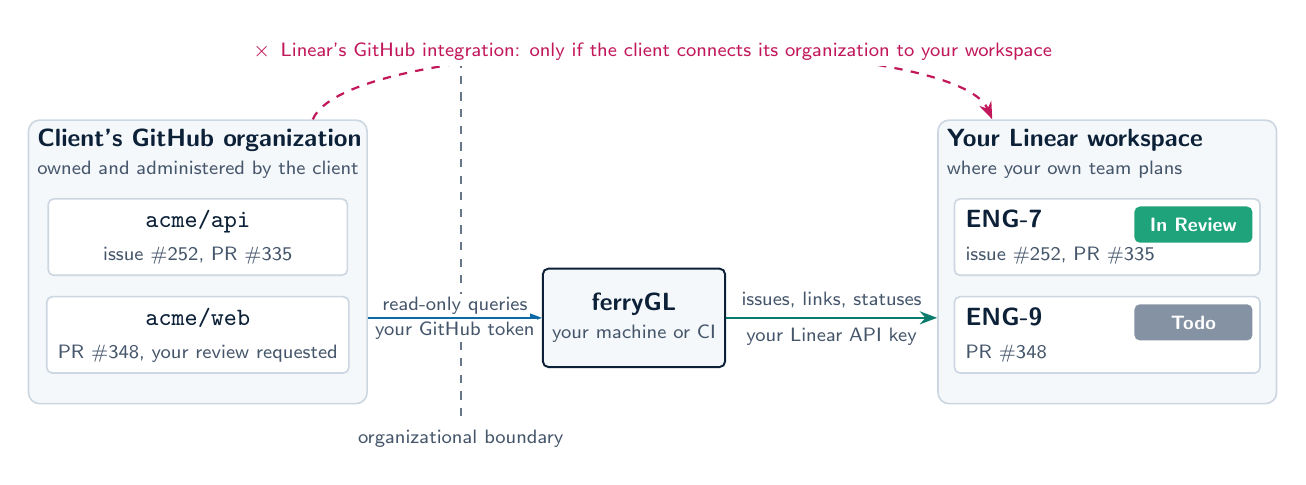
\begin{tikzpicture}[x=1cm, y=1cm]
  % The client's GitHub organization
  \node[region, minimum width=4.3cm, minimum height=3.6cm, anchor=south west] (client) at (0,0) {};
  \node[anchor=north west, font=\sffamily\small\bfseries] at (client.north west) {Client's GitHub organization};
  \node[anchor=north west, note] at ($(client.north west)+(0,-0.4)$) {owned and administered by the client};
  \node[box, minimum width=3.8cm, anchor=north] (repo1) at ($(client.north)+(0,-1.0)$)
    {\texttt{acme/api}\\[1pt]\scriptsize\color{fgMuted}issue \#252, PR \#335};
  \node[box, minimum width=3.8cm, anchor=north] (repo2) at ($(repo1.south)+(0,-0.25)$)
    {\texttt{acme/web}\\[1pt]\scriptsize\color{fgMuted}PR \#348, your review requested};

  % Your Linear workspace
  \node[region, minimum width=4.3cm, minimum height=3.6cm, anchor=south west] (linear) at (11.55,0) {};
  \node[anchor=north west, font=\sffamily\small\bfseries] at (linear.north west) {Your Linear workspace};
  \node[anchor=north west, note] at ($(linear.north west)+(0,-0.4)$) {where your own team plans};
  \node[box, minimum width=3.8cm, anchor=north, align=flush left, text width=3.6cm] (eng7)
    at ($(linear.north)+(0,-1.0)$)
    {\textbf{ENG-7}\\[1pt]\scriptsize\color{fgMuted}issue \#252, PR \#335};
  \node[review, minimum width=1.5cm, anchor=north east] at ($(eng7.north east)+(-0.1,-0.1)$) {In Review};
  \node[box, minimum width=3.8cm, anchor=north, align=flush left, text width=3.6cm] (eng9)
    at ($(eng7.south)+(0,-0.25)$)
    {\textbf{ENG-9}\\[1pt]\scriptsize\color{fgMuted}PR \#348};
  \node[todo, minimum width=1.5cm, anchor=north east] at ($(eng9.north east)+(-0.1,-0.1)$) {Todo};

  % The organizational boundary
  \draw[fgSubtle, dashed, line width=0.6pt] (5.5,-0.15) -- (5.5,4.3);
  \node[note, anchor=north] at (5.5,-0.2) {organizational boundary};

  % Linear's GitHub integration needs the client's administrators
  \draw[->, line width=0.8pt, fgRed, dashed] ($(client.north east)+(-0.7,0)$)
    .. controls +(0.5,1.15) and +(-0.5,1.15) .. ($(linear.north west)+(0.7,0)$)
    node[pos=0.5, fill=white, inner sep=2pt, note, text=fgRed] {\textbf{\(\times\)}\enspace
      Linear's GitHub integration: only if the client connects its organization to your workspace};

  % ferryGL's path, with your own credentials
  \node[stage, minimum width=2.1cm, minimum height=1.25cm, fill=fgSoft] (ferry) at (7.7,1.1)
    {\textbf{ferryGL}\\[-1pt]\scriptsize\color{fgMuted}your machine or CI};
  \draw[readflow] (client.east |- ferry) -- (ferry.west)
    node[pos=0.5, above, note, fill=white, inner sep=1pt] {read-only queries}
    node[pos=0.5, below, note, fill=white, inner sep=1pt] {your GitHub token};
  \draw[writeflow] (ferry.east) -- (linear.west |- ferry)
    node[pos=0.5, above, note] {issues, links, statuses}
    node[pos=0.5, below, note] {your Linear API key};
\end{tikzpicture}

  \caption{The gap \ferry{} fills. Linear's GitHub integration needs the client's
    organization to connect it, and a GitHub organization can be connected to only one Linear
    workspace. \ferry{} instead reads GitHub with the user's own token, read-only, and writes
    to the user's own Linear workspace with their own API key. Repository names and issue
    numbers here and throughout the paper are synthetic.}
  \label{fig:gap}
\end{figure}

People bridge the gap in one of three ways today. They copy issues and pull requests by
hand, and move each status again whenever something changes on GitHub: repetitive, manual
work of the kind site reliability engineering calls toil \cite{rau2016eliminating}, which
adds to the switching between tools and tasks that fragments developers' days
\cite{meyer2017work}. They ask a general-purpose AI agent to do it, since agents that
reason and call tools can drive both APIs; but the agent spends tokens on every run to reread
the same items and repeat the same moves, and its behavior is not guaranteed to be the same
twice \cite{ouyang2025empirical,
atil2025nondeterminism}. Or they ask the client to connect its organization, which is
often not theirs to ask.

\ferry{} takes a fourth route. It is a small command-line program that a person runs by
hand or on a schedule. Using only that person's GitHub token and Linear API key, it finds
the issues and pull requests they are part of in the repositories they list, gives each
one a Linear issue assigned to them and linked to GitHub, and keeps the status of that
issue in step with GitHub. It never writes to GitHub, never touches a teammate's Linear
issue, and never deletes anything. It follows the same rules on every run, shows each
change before making it, and spends no model tokens. An AI agent can run it too: instead of
doing the job itself, the agent runs \ferry, reads its plan, and spends its tokens on that
alone, \DelegationRatioHundredLow{} to \DelegationRatioHundredHigh{} times fewer on a
route of 100 items (\cref{sec:agents,sec:eval-agent}).

The design rests on one decision: \emph{the destination is the database}. Every Linear issue
that \ferry{} manages carries a link to its GitHub item, and the link's metadata records the
GitHub state that \ferry{} last acted on. Linear can find links by URL, so \ferry{} needs no
state of its own to find its earlier work; and because it compares GitHub with the recorded
state rather than with the Linear status, it moves a status only when something happens on
GitHub, and leaves the user's own edits alone in between.

\paragraph{Contributions.} This paper makes six contributions:
\begin{enumerate}[1.]
  \item The case for token-free automation of routine agent work, and a method to compare an
    agent doing a task itself, an agent delegating it to a token-free tool, and the tool alone:
    measure the task's reads and writes, and price them under bracketing assumptions
    (\cref{sec:agents,sec:eval-agent}).
  \item A statement of the problem of personal, cross-organization, one-way issue
    synchronization under least privilege, with seven requirements (\cref{sec:problem}).
  \item A stateless design that keeps synchronization state in the destination's link
    metadata, giving idempotent reruns and edge-triggered status updates that preserve
    manual edits (\cref{sec:design}).
  \item Rules that map a person's roles on GitHub to Linear issues, including pull requests
    that ride with the issue they fix and the adoption of issues the user made by hand
    (\cref{sec:design}).
  \item An implementation whose safety rests on eight explicit invariants, a pure planner,
    and a client interface that cannot express the forbidden writes, with a command-line
    interface that people and AI agents use alike (\cref{sec:implementation,sec:safety,sec:agents}).
  \item An evaluation with a randomized, model-based simulation that injects write failures,
    a validated request-cost model, a planner benchmark, and estimates of what an AI agent
    would spend in tokens, dollars and time doing the job itself and delegating it, on
    \CmpModels{} models from \CmpProviders{} providers, released with its scripts and data
    (\cref{sec:evaluation}).
\end{enumerate}

\section{Background and problem statement}
\label{sec:problem}

\subsection{GitHub and Linear}

On GitHub, an \emph{issue} is open or closed; a closed issue has a reason, such as
\emph{completed}, \emph{not planned} or \emph{duplicate}. A \emph{pull request} is open,
closed or merged, and an open pull request may be a draft. A person can be part of an item
in several ways: as its author, as an assignee, as a reviewer who has submitted a review, as
a requested reviewer, or as the author of one of its commits. A pull request can declare the
issues it closes with keywords such as \enquote{Fixes \#10} in its description
\cite{github2026linking}, and GitHub search finds issues and pull requests by author,
assignee, reviewer, requested reviewer and update date \cite{github2026searching}. \ferry{}
uses GitHub's GraphQL API \cite{graphql2025specification, hartig2018semantics}, whose
\code{search} field returns at most 1,000 results \cite{github2026publicschema}, and which
charges each query rate-limit points: the number of requests needed to fill every
connection, divided by 100, with a limit of 5,000 points per hour for a user
\cite{github2026graphqlratelimits}.

In Linear, an issue belongs to a team, has an assignee, and has a status drawn from the
team's workflow; each workflow state has a type, such as \emph{unstarted}, \emph{started},
\emph{completed} or \emph{canceled}. An issue can carry \emph{attachments}, which Linear
displays as links. An attachment has a URL, a title, a subtitle, and key--value metadata
whose \enquote{values can be any string or number}; attaching the same URL to the same
issue again updates the existing attachment, and the \code{attachmentsForURL} query returns
every attachment to a URL, with its issue \cite{linear2026attachments, linear2026schema}. A
personal API key acts as its owner \cite{linear2026gettingstarted}. This paper calls
attachments \emph{links}, as Linear's interface does.

\subsection{Problem statement}

A person has a GitHub account~$g$, which can read some repositories owned by others, and a
Linear user~$v$ in their own workspace. They choose \emph{routes}: each route names some
repositories and the Linear team (and, optionally, project) that their work there should go
to. The task is to maintain, in each route's team, one Linear issue assigned to~$v$ for each
GitHub item that $g$ is part of in the route's repositories, linked to the item, with a
status that follows the item's state on GitHub, subject to seven requirements:

\begin{description}[leftmargin=2.2em, style=sameline, font=\normalfont\bfseries]
  \item[R1] \textbf{Least privilege.} Use only the person's own credentials. Read GitHub,
    never write to it, and install nothing in the other organization
    \cite{saltzer1975protection}.
  \item[R2] \textbf{Respect for others' work.} Change only Linear issues assigned to~$v$, and
    never delete anything.
  \item[R3] \textbf{The person's edits win.} A status set by hand in Linear stays until
    something happens on GitHub.
  \item[R4] \textbf{Idempotence without local state.} A rerun never duplicates an issue or a
    link, and the program keeps no server, database or cache.
  \item[R5] \textbf{Data minimization.} Copy as little as possible from repositories that
    belong to someone else \cite{europeanunion2016gdpr, cavoukian2011privacy}.
  \item[R6] \textbf{No surprise writes.} Show every change before making it, and stop before
    reading or writing anything when the setup is wrong.
  \item[R7] \textbf{Token-free and deterministic.} Run no language model, so that a run costs
    API requests rather than model tokens, and the same inputs give the same plan.
\end{description}

\noindent Three things are explicitly \emph{not} goals: syncing in both directions, keeping
descriptions or comments in sync, and syncing every issue of a repository for a whole team,
which is what Linear's own integration does once it is installed. Reacting instantly is not
a goal either: webhooks would have to be created in the other organization's repositories,
which needs administrator access there \cite{github2026webhooks}, so \ferry{} polls.

\section{Design}
\label{sec:design}

\subsection{Overview}

A run of \ferry{} has five steps (\cref{fig:run}). It loads and validates the configuration,
then resolves every route's Linear setup: the API key's owner, the team, its workflow states,
and the project and label if configured. A missing team, state, project or label stops the
run before GitHub is read. Then, for each route, it reads GitHub, reads Linear, plans,
prints the plan and, only when run as \code{ferrygl sync \opt{apply}}, makes the planned
changes in Linear. Without \opt{apply}, a run performs every step except the writes.

\begin{figure}[t]
  \centering
  % The steps of a run, and what each reads from GitHub and Linear or writes to Linear.
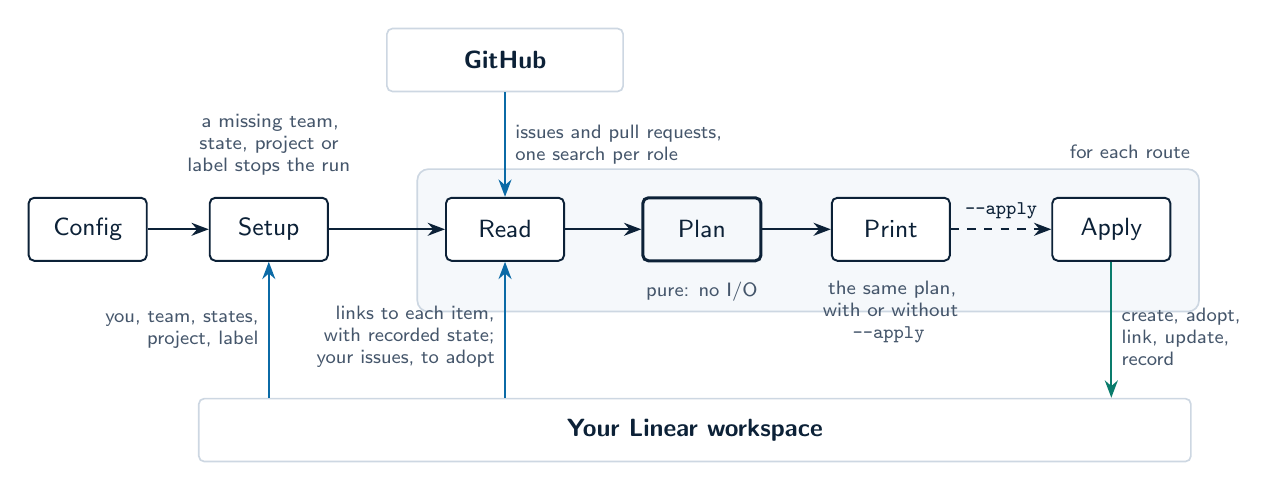
\begin{tikzpicture}[x=1cm, y=1cm]
  \node[stage] (config) at (0.75,0) {Config};
  \node[stage] (setup) at (3.05,0) {Setup};
  \node[stage] (read) at (6.05,0) {Read};
  \node[stage, fill=fgSoft, line width=1.1pt] (plan) at (8.55,0) {Plan};
  \node[stage] (print) at (10.95,0) {Print};
  \node[stage] (apply) at (13.75,0) {Apply};

  \draw[flow] (config) -- (setup);
  \draw[flow] (setup) -- (read);
  \draw[flow] (read) -- (plan);
  \draw[flow] (plan) -- (print);
  \draw[flow, dashed] (print) -- node[above, font=\ttfamily\scriptsize] {-{}-apply} (apply);

  % Per route
  \begin{scope}[on background layer]
    \node[region, fit={(read) (apply)}, inner xsep=10pt, inner ysep=14pt, yshift=-4pt] (route) {};
  \end{scope}
  \node[note, anchor=south east] at (route.north east) {for each route};

  % GitHub, read only
  \node[box, minimum width=3.0cm, minimum height=0.8cm, font=\sffamily\small\bfseries] (github) at (6.05,2.15) {GitHub};
  \draw[readflow] (github) -- node[right, note, align=left] {issues and pull requests,\\one search per role} (read);

  % Linear
  \node[box, minimum width=12.6cm, minimum height=0.8cm, anchor=west, font=\sffamily\small\bfseries]
    (linear) at (2.15,-2.55) {Your Linear workspace};
  \draw[readflow] (linear.north -| setup) -- node[left, note, align=right] {you, team, states,\\project, label} (setup);
  \draw[readflow] (linear.north -| read) -- node[left, note, align=right, pos=0.45] {links to each item,\\with recorded state;\\your issues, to adopt} (read);
  \draw[writeflow] (apply) -- node[right, note, align=left, pos=0.55] {create, adopt,\\link, update,\\record} (linear.north -| apply);

  % Notes
  \node[note, anchor=south, text width=2.6cm] at ($(setup.north)+(0,0.15)$)
    {a missing team, state, project or label stops the run};
  \node[note, anchor=north] at ($(plan.south)+(0,-0.12)$) {pure: no I/O};
  \node[note, anchor=north, text width=2.2cm] at ($(print.south)+(0,-0.12)$) {the same plan,\\with or without\\\texttt{-{}-apply}};
\end{tikzpicture}

  \caption{The steps of a run. GitHub is only read. All reads for a route happen before the
    plan, and all writes after it; the planner itself does no I/O. What a run writes to Linear
    is what the next run reads back.}
  \label{fig:run}
\end{figure}

\subsection{What is in scope}
\label{sec:scope}

For each route, \ferry{} runs one GitHub search per enabled \emph{role}
(\cref{tab:roles}), restricted to the route's repositories and, if configured, to items
updated since a given date. It merges the results into one item per URL that keeps every
role the person has on it. Each item has a \emph{kind}: \key{issue}, \key{pr} (a pull request
the person opened) or \key{involved} (someone else's pull request the person is part of). The
kind selects the title template and the status rules. Commenting on an item or being
mentioned in it does not bring it into scope, since that would pull in many items touched only
in passing.

\begin{table}[t]
  \centering\small
  \caption{Roles and the GitHub search behind each, for the login \code{alice}. Every search
    is also restricted to the route's repositories (\code{repo:acme/api}, or \code{user:acme}
    for every repository of an owner) and, with \code{since}, to \code{updated:>=}\emph{date}.}
  \label{tab:roles}
  \begin{tabularx}{\linewidth}{@{}l >{\raggedright\arraybackslash}X >{\ttfamily\footnotesize}l l@{}}
    \toprule
    Flag & Brings in & \normalfont\small Search & Kind \\
    \midrule
    \code{issues\_assigned} & Issues assigned to you & is:issue assignee:alice & \key{issue} \\
    \code{issues\_created} & Issues you created & is:issue author:alice & \key{issue} \\
    \code{prs\_created} & Pull requests you opened & is:pr author:alice & \key{pr} \\
    \code{prs\_assigned} & Others' pull requests assigned to you & is:pr assignee:alice -author:alice & \key{involved} \\
    \code{prs\_reviewed} & Others' pull requests you reviewed & is:pr reviewed-by:alice -author:alice & \key{involved} \\
    \code{review\_requests} & Others' pull requests where your review is requested & is:pr user-review-requested:alice -author:alice & \key{involved} \\
    \code{prs\_with\_commits} & Others' pull requests with your commits & is:pr -author:alice\normalfont\small, then a scan & \key{involved} \\
    \bottomrule
  \end{tabularx}
\end{table}

GitHub search has no qualifier for the author of a pull request's commits
\cite{github2026searching}, so the last role is the one expensive part of a run: \ferry{}
reads every pull request in scope that the person did not open, with the authors of its first
100 commits, and keeps those with a commit whose author GitHub links to the person's account.
\Cref{sec:eval-cost} measures what this costs.

\subsection{Homes, and state kept in the destination}
\label{sec:homes}

Each GitHub item has at most one \emph{home}: a Linear issue assigned to~$v$ that has a link
to the item's URL. \ferry{} finds homes by asking Linear for the links to each item's URL
(\code{attachmentsForURL}) and keeping the one on an issue assigned to~$v$. That is the whole
of its lookup: it needs no mapping table of its own, and a rerun after a crash, on another
machine, or months later finds the same homes. Because the lookup is by link and not by
team, a user may move a Linear issue to another team or project and \ferry{} still finds it,
as long as the new team uses the same status names.
Links on issues assigned to anyone else are ignored, so a teammate's issue that links the same
pull request is never touched, and reassigning an issue hands it off: if the item is still in
scope, the next run creates a new home for the user.

On each home's link, \ferry{} records what it needs to remember as flat metadata keys, which
fit Linear's string-or-number values (\cref{fig:home}). \key{ferrygl\_state} is the GitHub
state key \ferry{} last acted on, and \key{ferrygl\_synced\_at} the start of the run that
recorded it; \key{ferrygl\_kind} and the format version \key{ferrygl\_v} complete the record.
When \ferry{} updates a link it replaces only its own \key{ferrygl\_} keys and keeps any
others. These keys, like the state keys below, live in users' workspaces, so they are a
compatibility contract: renaming one would make every recorded link look changed.

\begin{figure}[t]
  \centering
  % A home: the Linear issue of acme/api#252, with the pull request that rides with it.
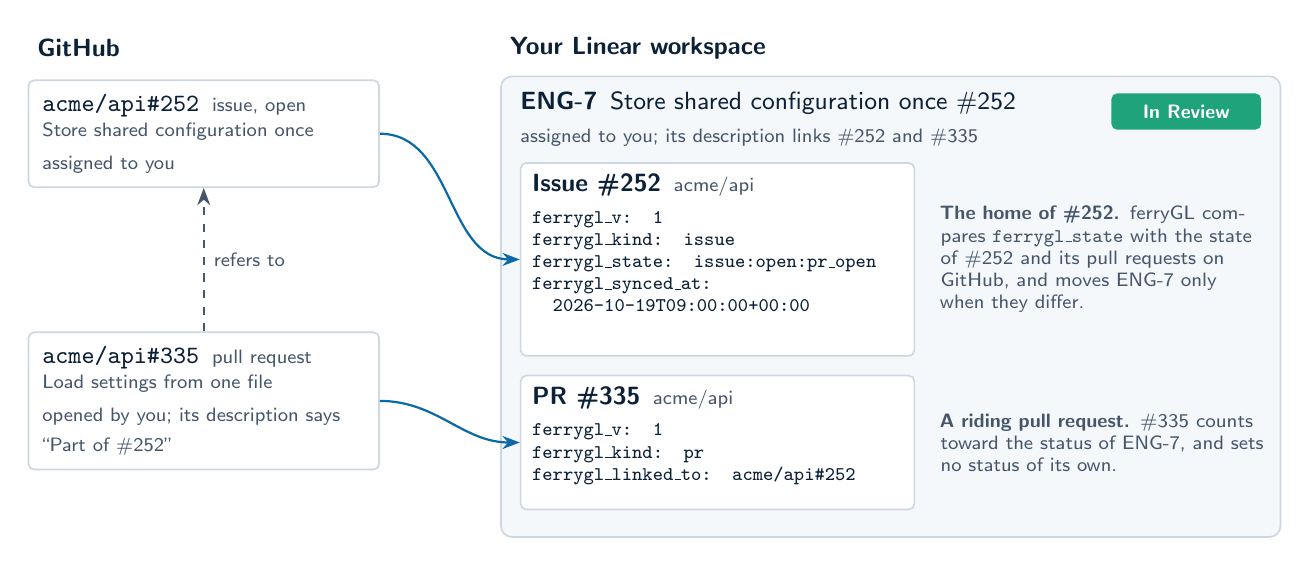
\begin{tikzpicture}[x=1cm, y=1cm,
    meta/.style={font=\ttfamily\scriptsize, text=fgNavy, anchor=north west, inner sep=0pt,
      align=left},
    card/.style={box, align=flush left, text width=4.1cm, inner sep=5pt}]
  % GitHub
  \node[font=\sffamily\small\bfseries, anchor=west] at (0,4.75) {GitHub};
  \node[card, anchor=north west] (issue) at (0,4.35)
    {\texttt{acme/api\#252}\enspace\scriptsize\color{fgMuted}issue, open\\[1pt]
     Store shared configuration once\\[1pt]
     \scriptsize\color{fgMuted}assigned to you};
  \node[card, anchor=north west] (pr) at (0,1.15)
    {\texttt{acme/api\#335}\enspace\scriptsize\color{fgMuted}pull request\\[1pt]
     Load settings from one file\\[1pt]
     \scriptsize\color{fgMuted}opened by you; its description says ``Part of \#252''};
  \draw[->, dashed, fgMuted, line width=0.6pt] (pr.north) -- node[right, note] {refers to} (issue.south);

  % Linear
  \node[font=\sffamily\small\bfseries, anchor=west] at (6.0,4.75) {Your Linear workspace};
  \node[region, anchor=north west, minimum width=9.9cm, minimum height=5.85cm] (lin) at (6.0,4.4) {};
  \node[anchor=north west, align=left, inner sep=0pt] at ($(lin.north west)+(0.25,-0.2)$)
    {\textbf{ENG-7}\enspace Store shared configuration once \#252\\[1pt]
     \scriptsize\color{fgMuted}assigned to you; its description links \#252 and \#335};
  \node[review, anchor=north east] at ($(lin.north east)+(-0.25,-0.22)$) {In Review};

  \node[box, anchor=north west, minimum width=5.0cm, minimum height=2.45cm] (link1) at (6.25,3.3) {};
  \node[anchor=north west, inner sep=0pt] at ($(link1.north west)+(0.15,-0.15)$)
    {\textbf{Issue \#252}\enspace\scriptsize\color{fgMuted}acme/api};
  \node[meta] at ($(link1.north west)+(0.15,-0.62)$)
    {ferrygl\_v: 1\\ferrygl\_kind: issue\\ferrygl\_state: issue:open:pr\_open\\
     ferrygl\_synced\_at:\\\quad 2026-10-19T09:00:00+00:00};
  \node[note, anchor=west, align=left, text width=4.1cm] at ($(link1.east)+(0.2,0)$)
    {\textbf{The home of \#252.} ferryGL compares \texttt{ferrygl\_state} with the state of
     \#252 and its pull requests on GitHub, and moves \mbox{ENG-7} only when they differ.};

  \node[box, anchor=north west, minimum width=5.0cm, minimum height=1.7cm] (link2) at (6.25,0.6) {};
  \node[anchor=north west, inner sep=0pt] at ($(link2.north west)+(0.15,-0.15)$)
    {\textbf{PR \#335}\enspace\scriptsize\color{fgMuted}acme/api};
  \node[meta] at ($(link2.north west)+(0.15,-0.62)$)
    {ferrygl\_v: 1\\ferrygl\_kind: pr\\ferrygl\_linked\_to: acme/api\#252};
  \node[note, anchor=west, align=left, text width=4.1cm] at ($(link2.east)+(0.2,0)$)
    {\textbf{A riding pull request.} \#335 counts toward the status of \mbox{ENG-7}, and sets
     no status of its own.};

  \draw[readflow] (issue.east) to[out=0, in=180] (link1.west);
  \draw[readflow] (pr.east) to[out=0, in=180] (link2.west);
\end{tikzpicture}

  \caption{A home and a riding pull request. ENG-7 is the home of issue \#252: its link
    records the GitHub state \ferry{} last acted on. Pull request \#335 refers to \#252, so
    instead of a Linear issue of its own it gets a link on ENG-7, marked
    \key{ferrygl\_linked\_to}.}
  \label{fig:home}
\end{figure}

\subsection{From GitHub state to Linear status}
\label{sec:states}

\ferry{} summarizes each item's position on GitHub as a \emph{state key}
$\sigma(i)$, one of sixteen strings such as \key{issue:open:pr\_open} or \key{pr:merged}
(\cref{fig:states}). For a pull request the key follows from its kind and state, and for
someone else's pull request also from the person's review roles: a pending review request
maps to \status{Todo}, even after an earlier review, because it is the person's turn again.
An issue's key also depends on the pull requests linked to it (\cref{sec:riders}): an
open issue whose linked pull request is open and ready for review is \status{In Review}, and
one whose linked pull requests are all drafts is \status{In Progress}.

Each key maps to one of five status categories (\status{Todo}, \status{In Progress},
\status{In Review}, \status{Done}, \status{Canceled}), whose names in the team's workflow are
configurable. The mapping has two forms. $\delta_{\text{new}}(\sigma)$ is the status of a
newly created Linear issue, and $\delta_{\text{chg}}(\sigma)$ the status to move to when the
state has changed. They agree everywhere except on \key{issue:open:pr\_merged}: the fix has
landed but the issue is still open, so a new Linear issue starts in \status{In Review},
while an existing one keeps its status, since the work is not done until the issue is
closed.

\begin{figure}[t]
  \centering
  % State keys, as recorded in ferrygl_state, and the Linear status each one leads to.
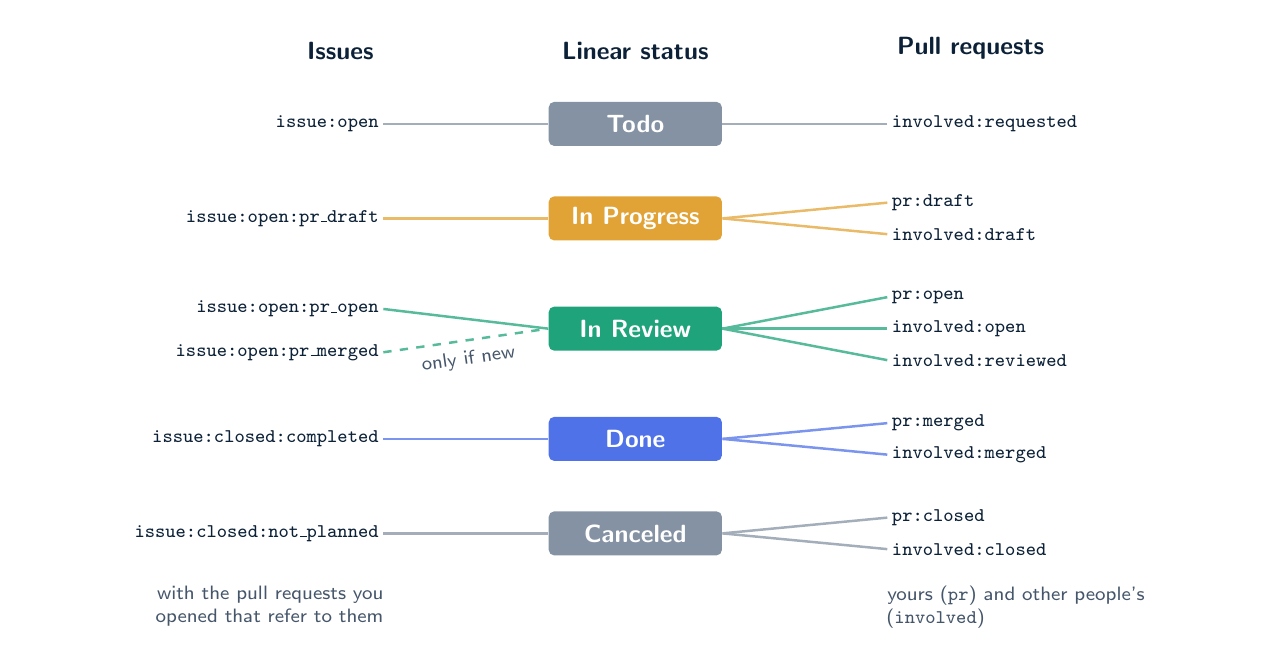
\begin{tikzpicture}[x=1cm, y=1cm,
    sk/.style={statekey, inner sep=1.5pt},
    edge/.style={line width=0.9pt, draw=#1!75},
    st/.style={minimum width=22mm, minimum height=5.6mm, font=\sffamily\small\bfseries}]
  % Statuses
  \node[todo, st] (todo) at (7.8,5.2) {Todo};
  \node[progress, st] (prog) at (7.8,4.0) {In Progress};
  \node[review, st] (rev) at (7.8,2.6) {In Review};
  \node[done, st] (done) at (7.8,1.2) {Done};
  \node[canceled, st] (canc) at (7.8,0.0) {Canceled};

  % Issues, with the user's pull requests that refer to them
  \foreach \key/\y/\to/\col in {
      issue:open/5.2/todo/stTodo,
      issue:open:pr\_draft/4.0/prog/stProgress,
      issue:open:pr\_open/2.85/rev/stReview,
      issue:closed:completed/1.2/done/stDone,
      issue:closed:not\_planned/0.0/canc/stCanceled} {
    \node[sk, anchor=east] (k) at (4.6,\y) {\key};
    \draw[edge=\col] (k.east) -- (\to.west);
  }
  \node[sk, anchor=east] (merged) at (4.6,2.3) {issue:open:pr\_merged};
  \draw[edge=stReview, dashed] (merged.east) -- node[below, sloped, note, pos=0.5] {only if new} (rev.west);

  % Pull requests: the user's own (pr) and other people's (involved)
  \foreach \key/\y/\to/\col in {
      involved:requested/5.2/todo/stTodo,
      pr:draft/4.2/prog/stProgress,
      involved:draft/3.8/prog/stProgress,
      pr:open/3.0/rev/stReview,
      involved:open/2.6/rev/stReview,
      involved:reviewed/2.2/rev/stReview,
      pr:merged/1.4/done/stDone,
      involved:merged/1.0/done/stDone,
      pr:closed/0.2/canc/stCanceled,
      involved:closed/-0.2/canc/stCanceled} {
    \node[sk, anchor=west] (k) at (11.0,\y) {\key};
    \draw[edge=\col] (k.west) -- (\to.east);
  }

  % Headings
  \node[font=\sffamily\small\bfseries, anchor=south east] at (4.6,5.9) {Issues};
  \node[note, anchor=north east, align=right] at (4.6,5.9) {};
  \node[font=\sffamily\small\bfseries, anchor=south] at (7.8,5.9) {Linear status};
  \node[font=\sffamily\small\bfseries, anchor=south west] at (11.0,5.9) {Pull requests};
  \node[note, anchor=north, text width=4.4cm, align=right] at (2.4,-0.55)
    {with the pull requests you opened that refer to them};
  \node[note, anchor=north, text width=4.4cm, align=left] at (13.2,-0.55)
    {yours (\texttt{pr}) and other people's (\texttt{involved})};
\end{tikzpicture}

  \caption{The sixteen state keys and the Linear status each leads to. For issues, the first
    matching rule wins, from closed to open. \key{issue:open:pr\_merged} sets a status only on
    a new Linear issue (dashed): when an existing issue's fix merges while the GitHub issue is
    still open, its status stays as it is.}
  \label{fig:states}
\end{figure}

\subsection{Edge-triggered updates: the person's edits win}
\label{sec:edges}

The central rule compares the current state key $s=\sigma(i)$ not with the Linear status, but
with the state key $\rho$ recorded on the item's home:
\begin{itemize}
  \item If $\rho = s$, nothing happens, whatever the Linear status is.
  \item If $\rho \neq s$ and $\rho$ is recorded, \ferry{} moves the status to
    $\delta_{\text{chg}}(s)$ (an \action{update}) and records~$s$. If the issue already has
    that status, or $\delta_{\text{chg}}(s)$ keeps the status, it only records~$s$ (a
    \action{record}).
  \item If no state is recorded ($\rho=\bot$), this is the link's \emph{first sync}: a link the
    user added by hand, or one \ferry{} just added to an issue the user made. \ferry{} then
    moves the status only to close the issue, to \status{Done} or \status{Canceled}, when
    GitHub says the work is done or canceled and the Linear issue is still open. It never
    reopens an issue, or moves it in any other way, on a first sync.
\end{itemize}
\Cref{alg:plan} gives the rule in full, with the cases of \cref{sec:riders,sec:adoption}.

A status therefore moves only on an \emph{edge} in the GitHub state, relative to a memory that
lives in the destination. \Cref{fig:timeline} contrasts this with a level-triggered sync,
which would compute the desired status from GitHub on every run and overwrite the person's
edits each time. Level-triggered reconciliation is the right model when the source of truth
should win continuously, as in the controllers of Borg, Omega and Kubernetes
\cite{burns2016borg}. Here two parties own different things: GitHub owns what happened on
GitHub, and the person owns their own tracker. Recording the last synchronized state and
comparing against it is how file synchronizers tell which replica changed
\cite{balasubramaniam1998file, pierce2004unison}. \ferry{} applies the same update detection
to the source only, and treats the Linear status as the person's between edges.

\begin{figure}[t]
  \centering
  % Edge-triggered status updates: ferryGL moves a status only when the GitHub state differs
% from the state recorded on the link. A level-triggered sync would undo the user's edits.
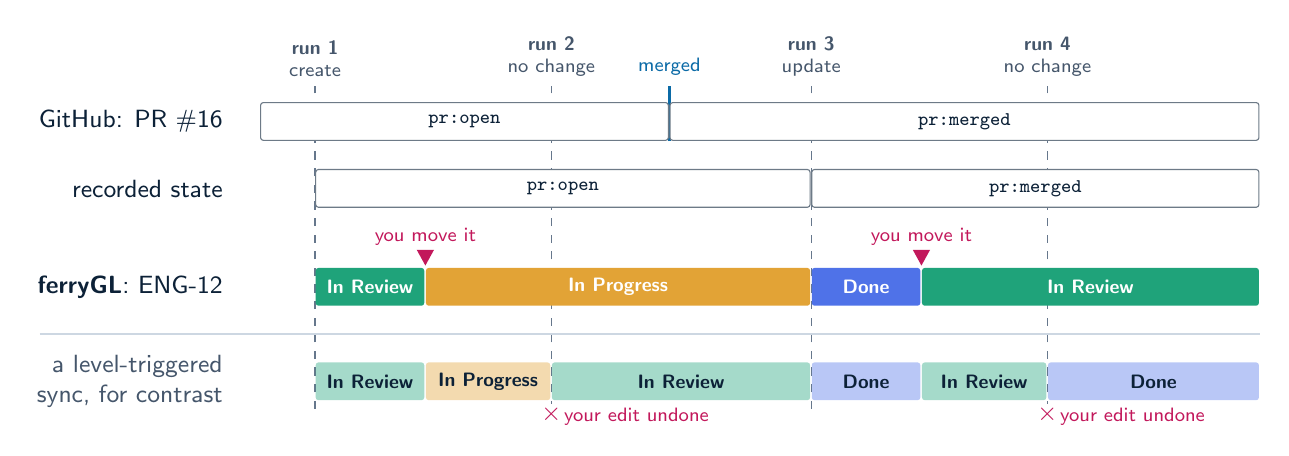
\begin{tikzpicture}[x=1cm, y=1cm,
    seg/.style={minimum height=4.8mm, inner sep=0pt, font=\sffamily\scriptsize\bfseries,
      text=white, rounded corners=1pt},
    ghost/.style={seg, fill opacity=0.4, text opacity=1, text=fgNavy},
    keyseg/.style={draw=fgNavy!60, fill=white, minimum height=4.8mm, inner sep=0pt,
      font=\ttfamily\scriptsize, rounded corners=1pt},
    lane/.style={font=\sffamily\small, anchor=east, align=right, text=fgNavy}]
  \newcommand{\seg}[5]{\node[#4, minimum width={(#3-#2)*1cm-0.6pt}, anchor=west] at (#2,#1) {#5};}

  % Runs, and what each one does
  \foreach \x/\n/\what in {3.9/1/create, 6.9/2/no change, 10.2/3/update, 13.2/4/no change} {
    \draw[fgSubtle, dashed, line width=0.5pt] (\x,-0.35) -- (\x,3.75);
    \node[note, anchor=south, align=center] at (\x,3.75) {\textbf{run \n}\\\what};
  }
  % Events between runs
  \draw[fgBlue, line width=0.8pt] (8.4,3.05) -- (8.4,3.75) node[above, note, text=fgBlue] {merged};
  \foreach \x in {5.3, 11.6} {
    \fill[fgRed] (\x,1.47) -- ++(-0.11,0.2) -- ++(0.22,0) -- cycle;
    \node[note, text=fgRed, anchor=south, inner sep=1pt] at (\x,1.68) {you move it};
  }

  % Lanes
  \node[lane] at (2.85,3.3) {GitHub: PR \#16};
  \node[lane] at (2.85,2.45) {recorded state};
  \node[lane] at (2.85,1.2) {\textbf{ferryGL}: ENG-12};
  \node[lane, text=fgMuted] at (2.85,0.0) {a level-triggered\\sync, for contrast};
  \draw[fgBorder, line width=0.5pt] (0.4,0.6) -- (15.9,0.6);

  \seg{3.3}{3.2}{8.4}{keyseg}{pr:open}
  \seg{3.3}{8.4}{15.9}{keyseg}{pr:merged}
  \seg{2.45}{3.9}{10.2}{keyseg}{pr:open}
  \seg{2.45}{10.2}{15.9}{keyseg}{pr:merged}

  \seg{1.2}{3.9}{5.3}{seg, fill=stReview}{In Review}
  \seg{1.2}{5.3}{10.2}{seg, fill=stProgress}{In Progress}
  \seg{1.2}{10.2}{11.6}{seg, fill=stDone}{Done}
  \seg{1.2}{11.6}{15.9}{seg, fill=stReview}{In Review}

  \seg{0.0}{3.9}{5.3}{ghost, fill=stReview}{In Review}
  \seg{0.0}{5.3}{6.9}{ghost, fill=stProgress}{In Progress}
  \seg{0.0}{6.9}{10.2}{ghost, fill=stReview}{In Review}
  \seg{0.0}{10.2}{11.6}{ghost, fill=stDone}{Done}
  \seg{0.0}{11.6}{13.2}{ghost, fill=stReview}{In Review}
  \seg{0.0}{13.2}{15.9}{ghost, fill=stDone}{Done}
  \foreach \x in {6.9, 13.2} {
    \node[fgRed, font=\sffamily\small\bfseries, fill=white, inner sep=0.5pt] at (\x,-0.42) {\(\times\)};
    \node[note, text=fgRed, anchor=north west, inner sep=1pt] at (\x+0.12,-0.3) {your edit undone};
  }
\end{tikzpicture}

  \caption{Edge-triggered updates for one pull request and its Linear issue. Run~1 creates
    ENG-12 in \status{In Review} and records \key{pr:open}. The user moves it to
    \status{In Progress}; run~2 sees the recorded state still matches GitHub and changes
    nothing. Run~3 sees the merge and moves it to \status{Done}. The user then reopens it, and
    run~4 leaves it alone. A level-triggered sync (bottom) would undo both edits.}
  \label{fig:timeline}
\end{figure}

\begin{algorithm}[t]
  \caption{Planning one item $i$, with its linked pull requests $L$ and riders $R$
    (\cref{sec:riders}). $A(u)$ are the links to URL $u$ returned by Linear, $C$ the user's
    issues in the route's team, and $v$ the user.}
  \label{alg:plan}
  \small
  \begin{algorithmic}[1]
    \State $s \gets \sigma(i, L)$
    \State $h \gets$ the first link in $A(\mathit{url}(i))$ on an issue assigned to $v$, if any
      \Comment{the home}
    \If{$h$ exists}
      \State $\rho \gets$ the state recorded on $h$, or $\bot$
      \If{$\rho \neq s$}
        \If{$\rho = \bot$} \Comment{first sync: only close}
          \State $c \gets \delta_{\text{chg}}(s)$ if it is \status{Done} or \status{Canceled}
            and $h$'s issue is open, else none
        \Else
          \State $c \gets \delta_{\text{chg}}(s)$
        \EndIf
        \State emit \action{update}$(h, c)$ if $c$ differs from the issue's status, else
          \action{record}$(h)$; both record $s$ on $h$
      \EndIf
      \State emit \action{link}$(r)$ for each $r \in R$ not yet linked to $h$'s issue
    \Else
      \State $M \gets \{\, m \in C$ unclaimed, mentioning $i$ or a rider, and linked to no other
        GitHub item $\}$
      \If{$|M| > 1$}
        \State emit \action{skip}$(i, M)$ \Comment{the user decides}
      \ElsIf{$|M| = 1$}
        \State emit \action{adopt}$(i, m)$ under the first-sync rule, and claim $m$
      \Else
        \State emit \action{create}$(i)$ with status $\delta_{\text{new}}(s)$, linking $i$ and $R$
      \EndIf
    \EndIf
  \end{algorithmic}
\end{algorithm}

Two properties follow, and \cref{sec:evaluation} tests both.

\paragraph{Edits persist.} If a run completes its writes, every home it touched records the
state key it acted on. If, by the next run, the key \ferry{} computes for an item is
unchanged, the first branch applies and the home's status is left alone, whatever the user
did to it in between. (The key of an issue depends on its linked pull requests, so a new
review request or a merge is an edge; \cref{sec:eval-order} shows one case where the key
changes without anything new on GitHub.)

\paragraph{Quiescence.} If neither GitHub nor Linear changes after a run that completed its
writes, the next run plans no writes: every item in scope has a home that records its current
key, and every rider is linked. Reruns are therefore safe to schedule as often as wanted.

\subsection{Pull requests that ride with an issue}
\label{sec:riders}

An issue and the pull request that fixes it are one piece of work. When a pull request the
person opened refers to one of their synced issues in the same route, it does not get a
Linear issue of its own: it \emph{rides} with the issue, and \ferry{} links it to the issue's
home instead, with \key{ferrygl\_linked\_to} naming the issue (\cref{fig:home}). A pull
request refers to an issue when GitHub lists the issue as one it will close, or when its title
or description mentions it as \code{\#252}, \code{acme/api\#252} or by URL. The issue's state
key then accounts for its linked pull requests, so the home follows the issue and its fix
together: \status{In Progress} while the fix is a draft, \status{In Review} when it is open,
and \status{Done} only when the issue itself is closed. The rider's link sets no status of
its own, so each Linear issue has one status source.

A few cases need care. A pull request that already had a home of its own before it referred to
the issue keeps it, and still counts toward the issue's status. Conversely, an issue that has
no home while its pull request does \emph{joins} the pull request's home, as long as the pull
request refers to no other synced issue. A rider's link stays when the reference is later
edited out, and it keeps counting toward the issue's status. When the issue leaves the
person's scope (they are unassigned, say) while the pull request is still in it, the issue's
home stays as it is: the rider does not move it on its own. Someone else's pull request always
gets its own home, even if it refers to the person's issue. Finally, a pull request that refers
to several of the person's issues rides with each of them, so its URL is linked from each
of their Linear issues, as a rider; it is still the home of none.

\subsection{Adopting issues the person made by hand}
\label{sec:adoption}

People often create a Linear issue for a GitHub item themselves before they install \ferry.
Before creating a new issue, \ferry{} therefore looks for one of the person's issues in the
route's team that already mentions the item: its URL in the description or in a link, or, for
a route with a single repository, a title ending in \code{\#}\emph{number} with no link to any
other GitHub item. A candidate already linked to a different GitHub item, or already home to
another item, never matches. Exactly one match is \emph{adopted}: \ferry{} adds its link and
applies the first-sync rule, so the adopted issue's status moves only to close it. Several
matches are \emph{skipped}, with their identifiers: the person adds the link to the right one
by hand, and the next run picks it up.

\subsection{Writes, failures and retries}
\label{sec:failures}

Each change is applied in a fixed order: the status first, then \ferry's comment (if comments
are on), then the links. The recorded state therefore changes last: if the status update or
the comment fails, the old state stays recorded, and the next run plans the same change again.
Each change is applied independently, so one failure does not stop the others; the run then
exits with status~1.

Retries follow the idempotency of each request (\cref{tab:retries}) \cite{helland2012idempotence,
fielding2022rfc9110}. Rate-limited responses (HTTP 429 \cite{nottingham2012rfc6585}, or GitHub's
403 with \code{Retry-After}) are always retried, after the requested wait. Network errors,
timeouts and HTTP 502, 503 and 504 are retried only for idempotent requests: every read, a
status update, and a link create or update, which Linear makes idempotent per issue and URL
\cite{linear2026attachments}. Creating an issue or a comment is not idempotent: if the
connection fails, Linear may have created it anyway. \ferry{} reports the error instead of
retrying. If the issue was created, the next run finds it through the GitHub URL in its
description and adopts it, so no duplicate is created; a comment, however, may be posted twice.
Linear's create inputs accept an identifier chosen by the client \cite{linear2026schema}, which
could make these retries safe as well (\cref{sec:limitations}).

\begin{table}[t]
  \centering\small
  \caption{Retry policy. Each request gets up to three attempts. Waits honor
    \code{Retry-After}, up to 60~seconds, and are otherwise 2 and then 4~seconds. A request
    times out after 30~seconds, which counts as a network error.}
  \label{tab:retries}
  \begin{tabularx}{\linewidth}{@{}X >{\centering\arraybackslash}p{3.4cm} >{\centering\arraybackslash}p{4.2cm}@{}}
    \toprule
    Request & Rate limited (429, or 403 with \code{Retry-After}) & Network error, timeout, or 502, 503, 504 \\
    \midrule
    GitHub and Linear reads & retried & retried \\
    \code{issueUpdate}, \code{attachmentCreate}, \code{attachmentUpdate} & retried & retried \\
    \code{issueCreate}, \code{commentCreate} & retried & reported; adopted or retried next run \\
    \bottomrule
  \end{tabularx}
\end{table}

\section{Implementation}
\label{sec:implementation}

\ferry{} is a Python package of about 1,900 lines in eight main modules
(\cref{tab:modules}), with one runtime dependency, the HTTP client HTTPX
\cite{encode2024httpx}. It supports Python 3.11 and later. Its structure follows the
\enquote{functional core, imperative shell} pattern \cite{bernhardt2012functional,
moseley2006tar}: \code{plan.py} is a pure function from the GitHub items, the Linear links and
candidates, and the configuration to a list of changes, and everything that talks to the
network lives around it. All types passed between modules are frozen dataclasses.

\begin{table}[t]
  \centering\small
  \caption{Modules of \ferry{} \version, with their length in lines.}
  \label{tab:modules}
  \begin{tabularx}{\linewidth}{@{}l X r@{}}
    \toprule
    Module & Responsibility & Lines \\
    \midrule
    \code{plan.py} & Pure planning: GitHub items and Linear state to changes; state keys & 464 \\
    \code{sync.py} & \code{check} and \code{sync}: resolve routes, plan, print, apply & 318 \\
    \code{config.py} & Parse and validate \code{ferrygl.toml} into frozen dataclasses & 288 \\
    \code{linear.py} & Linear GraphQL reads, and the five mutations \ferry{} uses & 279 \\
    \code{github.py} & Tokens, one search per role, the commit scan, references & 272 \\
    \code{model.py} & Shared types: items, Linear issues, links, changes & 124 \\
    \code{cli.py} & Arguments, the Linear API key, exit statuses & 92 \\
    \code{\_http.py} & JSON over HTTP with retries, for both clients & 81 \\
    \bottomrule
  \end{tabularx}
\end{table}

\paragraph{Configuration.} The configuration is one TOML file \cite{prestonwerner2021toml}
(\cref{app:config}). Only the routes are required. Unknown tables and keys are errors, so a
misspelled setting cannot be silently ignored, and every error names the file and the
setting. A JSON Schema \cite{wright2018jsonschema, wright2018jsonschemavalidation} published
on the project's website gives editors completion and inline checks; a test keeps it in step
with the parser.

\paragraph{Commands and output.} \code{ferrygl check} confirms that the Linear key works,
that the GitHub token can see every repository, and that each route's team, states, project
and label exist; it writes nothing. \code{ferrygl sync} prints the plan, one line per change,
and \code{ferrygl sync \opt{apply}} prints the same plan and makes it:
\begin{lstlisting}
acme/api#252  issue     update  ENG-7 Todo -> In Review
acme/api#335  pr        link    -> ENG-7
acme/api#360  issue     create  "Cache the session lookup #360" -> Todo
acme/api#348  involved  adopt   -> ENG-9
4 changes (1 create, 1 adopt, 1 link, 1 update). Run with --apply to make them.
\end{lstlisting}
The exit status is 0 when everything worked, 1 when a route could not be read or a write
failed, 2 for a setup or configuration error (in which case nothing was read from GitHub or
written to Linear), and 130 when interrupted. With comments turned on, every change also
posts a Linear comment that starts with the marker \code{(BY-FGL)}, so people can tell
\ferry's changes from their own and filter on them.

\paragraph{Requests.} Per route, a run makes one GitHub query for the token's login, then one
paged search per enabled role, at 50 results per page, or 25 pull requests per page for the
commit scan. On the Linear side, it looks up the user, each route's team, states, project and
label, then the links to up to 25 URLs per request, and, only when some item has no home yet,
the user's issues in the team, 50 per page. With \opt{apply}, each write is one request.
Linear allows 2,500 requests an hour for an API key \cite{linear2026ratelimiting}; a first run
that creates a few hundred issues uses a noticeable share of that, and later runs write only
what changed.

\paragraph{Tests.} The repository has 155 tests that run in under a second. Each planning
test states a scenario in plain terms (what is on GitHub, what is in Linear, the expected
changes); the clients are tested against \code{httpx.MockTransport}; and \code{check} and
\code{sync} run end to end against fakes. All test data is synthetic.

\section{Safety and privacy}
\label{sec:safety}

\ferry{} usually runs in repositories that belong to someone else, often private ones whose
contents are covered by an agreement, so its safety rules matter more than its features. The
repository's contributor guide states them as eight invariants, which human contributors and
coding agents alike must not break without the project owner's decision.
\Cref{tab:invariants} lists each one with the mechanism that enforces it and the evidence from
\cref{sec:evaluation}.

\begin{table}[t]
  \centering\small
  \caption{The eight invariants, how the design enforces them, and the evaluation evidence.}
  \label{tab:invariants}
  \begin{tabularx}{\linewidth}{@{}>{\raggedright\arraybackslash}p{3.35cm} >{\raggedright\arraybackslash}X >{\raggedright\arraybackslash}p{3.6cm}@{}}
    \toprule
    Invariant & Mechanism & Evidence \\
    \midrule
    I1.\ GitHub is read-only & The GitHub client only sends GraphQL queries & No mutation among all requests (\cref{sec:eval-cost}) \\
    I2.\ Only the user's Linear issues; nothing deleted or rewritten & Writes target homes or new issues assigned to the user; the Linear client has no delete, and its update sets only the status & \emph{ownership} (\cref{tab:sim}) \\
    I3.\ The user's edits win & Edge-triggered updates against the recorded state; first syncs only close & \emph{status source}, \emph{edits win} \\
    I4.\ One home per item, one status source per Linear issue & Lookup by link; claimed candidates; riders set no status & \emph{one home}, \emph{coverage} \\
    I5.\ Idempotent reruns & Homes found by link; only idempotent requests retried & \emph{quiescent}, \emph{recovery} \\
    I6.\ A pure planner & All reads before planning, all writes after & \emph{order independent} (one finding) \\
    I7.\ Copy as little as possible & Only titles, numbers, repositories, URLs, states and roles by default & \emph{minimal data} \\
    I8.\ No surprise writes & Preview by default; setup checked before reading GitHub & \emph{dry run} \\
    \bottomrule
  \end{tabularx}
\end{table}

\paragraph{Safety by interface.} Two invariants hold by construction rather than by care. The
GitHub client has no code path that sends a mutation. The Linear client exposes exactly five
mutations: \code{issueCreate}, \code{issueUpdate} with only a state, \code{attachmentCreate},
\code{attachmentUpdate} and \code{commentCreate}. No method can delete an issue, a link or a
comment, or edit an issue's title or description or a comment, so no bug in the planner can
make \ferry{} do so.

\paragraph{Credentials.} \ferry{} sends the GitHub token only to \code{api.github.com} and the
Linear key only to \code{api.linear.app}, and stores neither. A read-only GitHub token is
enough, and preferred; some organizations must approve fine-grained tokens before they can
read their repositories, which \code{ferrygl check} reports as a repository it cannot see.
The Linear key acts as the user, so \ferry's own rules, not the key's scope, keep it to the
user's issues; a key with limited permissions must still allow the writes \ferry{} makes.

\paragraph{What reaches Linear.} By default, \ferry{} writes the GitHub title and number (the
title template is configurable, and can leave the title out), the repository, the item's URL,
its state key, and the user's role as implied by the kind. It reads descriptions to find the
issues a pull request refers to, but copies them only if the user turns that on, once, when
the issue is created. It never copies GitHub comments, reviews, labels, code, or other
people's names or logins, including the authors of pull requests and commits. Its own
comments name only GitHub items, states and Linear status names. It keeps nothing on the
user's machine: no database, cache or log file of its own.

\section{Token-free automation for AI agents}
\label{sec:agents}

Many people who would use \ferry{} already work with an AI agent. An agent asked to keep
Linear in step with GitHub can do that job in two ways. It can do the job itself: search
GitHub for each role, look up each item in Linear, apply the rules of \cref{sec:design}, and
make the writes, reading every item on every run. Or it can delegate the job to a token-free
tool: run \code{ferrygl sync}, read the plan, run \code{ferrygl sync \opt{apply}}, and report.
Its tokens then go to what \ferry{} prints, a line per change and \code{No changes.} on a
quiet run, instead of to every item in scope. \Cref{sec:eval-agent} measures the difference:
on a route of 100 items, \DelegationRatioHundredLow{} to \DelegationRatioHundredHigh{}
times fewer tokens, and on 800 items \DelegationRatioEightHundredLow{} to
\DelegationRatioEightHundredHigh{} times fewer.

\paragraph{An interface agents can use.} \ferry{} needs nothing agent-specific: any agent
that can run a command can use it, through the same interface a person uses. Three of its
properties make that safe and cheap. A run previews by default: \code{ferrygl sync} writes
nothing, so an agent can show the plan to its user, or check it, before it runs
\code{ferrygl sync \opt{apply}}. The output is compact and regular: one line per change, with
the item, its kind, the action and its details, then a one-line summary, and every
\action{skip} line says what decision it needs. And the exit status says what happened: 0 when
everything worked, 1 when a route or a write failed, 2 when the setup is wrong and nothing
was read or written, and 130 when interrupted. \ferry's documentation has a page for agents,
with instructions a user can give their agent, and its website publishes an \code{llms.txt}
index of the documentation for language models \cite{howard2024llmstxt}. Instructions as short
as these are enough:
\begin{lstlisting}
To sync my GitHub work into Linear, run `ferrygl sync` and show me the plan.
Run `ferrygl sync --apply` only after I approve it. If a line says skip,
tell me what ferryGL needs. If the exit status is 2, report the error and stop.
Never change GitHub or Linear yourself to do this.
\end{lstlisting}

\paragraph{Least privilege for agents.} Delegating also narrows what an agent can do. An agent
whose only access to GitHub and Linear is \ferry{} cannot write to GitHub, change a
teammate's Linear issue, or delete anything, whatever it is asked or gets wrong: the
invariants of \cref{tab:invariants} hold for every caller, and \ferry's preview shows every
change first \cite{saltzer1975protection}. The agent needs no GitHub or Linear tools of its
own.

\paragraph{A general pattern.} The same split applies wherever an agent is asked to do
routine, rule-based work again and again: keeping trackers in step, triage by fixed rules,
recurring reports. Once a task's rules are known, writing them into a program once moves the
task's marginal cost from inference to API requests, and makes its behavior repeatable. This
complements tool-using agents \cite{schick2023toolformer, wang2024codeact} and agents that
write tools for themselves \cite{cai2024tool}: the tool here is written once, tested, and
shared, and the agent's role is to decide when to call it and to read what it reports. It is
an instance of the compound AI systems that combine models with conventional components
\cite{zaharia2024compound}; it complements other ways of reducing inference cost, such as
routing requests to cheaper models \cite{chen2024frugalgpt}; and it answers calls to weigh
agents' cost alongside their accuracy \cite{kapoor2025agents, xia2025agentless} and to count
efficiency as a goal \cite{schwartz2020green}.

\section{Evaluation}
\label{sec:evaluation}

The evaluation asks four questions. Do the safety invariants hold over long, random
histories in which GitHub changes, the user edits Linear, teammates link the same items, and
writes fail (\cref{sec:eval-sim})? How many requests and rate-limit points does a run cost,
and what dominates (\cref{sec:eval-cost})? Does the planner scale (\cref{sec:eval-planner})?
And what would an AI agent spend to do the same job, by itself or by delegating it to
\ferry, and how does that vary across models and providers
(\cref{sec:eval-agent,sec:eval-models})?
The scripts and their output are in the repository, under \code{docs/paper/}
(\cref{app:reproduce}).

\subsection{Randomized, model-based simulation}
\label{sec:eval-sim}

\paragraph{Method.} The simulation runs \ferry's own reading, planning and writing code,
unchanged, against two in-memory stand-ins with the same methods as its GitHub and Linear
clients. The GitHub stand-in answers each role's search from a model of issues and pull
requests, in the shape of GitHub's GraphQL nodes, so \ferry's result parsing and reference
detection run too. The Linear stand-in keeps issues, links and comments, and follows Linear's
documented behavior: links are returned by URL across the workspace, up to 20 per URL, and
attaching a URL an issue already has updates that link. As in property-based testing
\cite{claessen2000quickcheck}, each scenario is generated at random from a seed: one or two
repositories, a random configuration (each role on with probability 0.85, comments on or
off), and a few initial items. Then, for \SimSteps{} steps, random events happen and \ferry{}
runs. GitHub events open and close issues, open, ready, draft, merge, close and reopen pull
requests, request, give and withdraw reviews, assign and unassign the user, add and remove
references, and push commits. Linear events have the user move statuses, hand issues to a
teammate, link items by hand, and write issues that mention items, and have a teammate link
the same items and the user add their own metadata to \ferry's links. Three in ten steps
change only Linear. Each step runs \ferry{} four ways: a preview, an apply in which
\SimFaultRate{} of writes fail (half of them \emph{lost}, reaching Linear but losing their
response, and half \emph{rejected}), a clean recovery run if any write failed, and a final
clean rerun.

After every run, the simulation checks the properties of \cref{tab:sim} against the stand-ins'
state and the writes \ferry{} sent. GitHub descriptions in the model carry a secret marker and
mention other users, so \emph{minimal data} can check that no write carries either, and that no
comment carries a GitHub title. \emph{Order independent} is a metamorphic relation
\cite{chen1998metamorphic, chen2018metamorphic}: planning the same inputs with every list of
Linear lookup results reversed must give the same changes, since Linear promises no particular
order.

\paragraph{Results.} \SimScenarios{} scenarios produced \SimEvents{} events, \SimRuns{} runs
and \SimWrites{} writes, of which \SimFaultsInjected{} failed. The plans included
\SimActionCreate{} creates, \SimActionUpdate{} updates, \SimActionLink{} links,
\SimActionRecord{} records, \SimActionAdopt{} adoptions and \SimActionSkip{} skips. The whole
simulation takes about ten seconds. \Cref{tab:sim} shows the results: every safety property
held in every check. Write failures left \SimOrphans{} Linear issues created without their
links; the next clean run adopted all \SimOrphansAdopted{} of them through the URL in their
description, and every recovery converged in one run.

\begin{table}[t]
  \centering\small
  \caption{Properties checked by the simulation, how many times each was checked, and how
    many checks failed. A check is one evaluation of the property on one run's state, writes
    or plan.}
  \label{tab:sim}
  \begin{tabularx}{\linewidth}{@{}l X r r@{}}
    \toprule
    Property & Statement & Checks & Failed \\
    \midrule
    dry run & A run without \opt{apply} writes nothing & \SimChecksDryRun & \SimViolationsDryRun \\
    quiescent & A rerun with nothing new on GitHub or in Linear writes nothing & \SimChecksQuiescent & \SimViolationsQuiescent \\
    one home & Each GitHub item is linked as a home from at most one of the user's issues & \SimChecksOneHome & \SimViolationsOneHome \\
    ownership & Every write targets an issue assigned to the user & \SimChecksOwnership & \SimViolationsOwnership \\
    status source & A status moves only with a new recorded state, or to close on a first sync & \SimChecksStatusSource & \SimViolationsStatusSource \\
    edits win & After a step that changed only Linear, every status the user set is still set, unless a first sync closed the issue & \SimChecksEditsWin & \SimViolationsEditsWin \\
    coverage & Every item in scope is linked from one of the user's issues, unless it, or the issue it rides with, was skipped & \SimChecksCoverage & \SimViolationsCoverage \\
    consistent & A pull request's home records its current state and, unless the user moved it, has the status \cref{fig:states} gives & \SimChecksConsistent & \SimViolationsConsistent \\
    foreign metadata & Metadata keys that are not \ferry's survive every update & \SimChecksForeignMetadata & \SimViolationsForeignMetadata \\
    minimal data & No write carries a description or another user's login, and no comment a title & \SimChecksMinimalData & \SimViolationsMinimalData \\
    recovery & After failed writes, one clean run succeeds and converges & \SimChecksRecovery & \SimViolationsRecovery \\
    \midrule
    order independent & The plan does not depend on the order of Linear's lookup results & \SimChecksOrderIndependent & \SimViolationsOrderIndependent \\
    \bottomrule
  \end{tabularx}
\end{table}

\paragraph{A finding: order dependence.}
\label{sec:eval-order}
The metamorphic check failed in \SimViolationsOrderIndependent{} of \SimChecksOrderIndependent{}
non-trivial checks, all with the same cause. A pull request that refers to two of the user's
issues rides with both, so its URL is linked from both of their Linear issues. If one reference
is later edited out, the planner looks up the pull request's links and takes the first one on
the user's issue as the pull request's own. When that first link is on the issue it still
refers to, the pull request rides with that issue only, and stops counting toward the other
issue's status: that issue's state key changes, say from \key{issue:open:pr\_open} to
\key{issue:open}, and its Linear issue moves back to \status{Todo}. When the first link is
on the other issue, the sticky-link rule of \cref{sec:riders} applies, as documented, and
nothing moves. Since Linear does not promise an order for these results, the outcome is not
determined. The case is narrow (a pull request that refers to several of the user's issues
and then drops one reference) and moves only the status of the user's own issue, but it
breaks the documented rule and the purity of the planner's inputs. A fix is to choose among
a pull request's links deterministically, preferring a link on the home of an issue it still
refers to, and to keep counting the pull request toward the status of every issue whose home
has its link.

\subsection{Request cost}
\label{sec:eval-cost}

\paragraph{Method.} The cost experiment runs \ferry's real GitHub client against a mock of
GitHub's GraphQL endpoint, built on \code{httpx.MockTransport}, that pages results as GitHub
does and stops at 1,000 results per search. The repository holds a fixed set of the user's own
items (12 issues, 8 pull requests) and a growing number of other people's pull requests; one in
ten requests the user's review, one in ten was reviewed by them, one in twenty is assigned to
them, and one in twenty has one of their commits. For each size, the experiment counts the
requests \ferry{} sends and the rate-limit points GitHub would charge, using GitHub's
documented cost formula \cite{github2026graphqlratelimits}. A search page of 50 results with
their closing references costs 1 point. A commit-scan page of 25 pull requests, each with 100
commits of up to 5 authors, needs $1 + 25 + 25 + 25 \times 100 = 2{,}551$ requests to fill, and
costs 26 points.

\paragraph{Results.} The request count \ferry{} sent matched a closed-form model at every size,
and none of the requests was a mutation. \Cref{fig:cost} shows the result. Without the commit
scan, a route with 1,000 other pull requests in scope costs 9 requests and 9 points. With it,
the same route costs 49 requests and 1,049 points, about a fifth of a user's hourly 5,000; the
scan accounts for 40 of the requests and 1,040 of the points. Beyond 1,000 pull requests,
GitHub's limit on search results truncates the scan: the cost stops growing, but pull requests
past the 1,000th are no longer checked, so some of the user's commits go unseen. This is why
\ferry's documentation recommends setting \code{since}, which bounds every search by update
date, and turning \code{prs\_with\_commits} off when the role is not needed.

\begin{figure}[t]
  \centering
  % GitHub requests and rate-limit points for one route, from data/github-cost.csv
% (evaluation/costs.py).
\begin{tikzpicture}
  \begin{groupplot}[ferrygl,
      group style={group size=2 by 1, horizontal sep=1.9cm},
      width=7.6cm, height=5.4cm,
      xmin=0, xmax=1600, xtick={0,400,800,1200,1600},
      xlabel={other people's pull requests in scope},
      % The samples are dense below 200, so the lines carry no marks.
      every axis plot/.append style={mark=none},
    ]
    \nextgroupplot[ylabel={GraphQL requests}, ymin=0, ymax=60,
      legend to name=costlegend, legend columns=2,
      legend style={/tikz/every even column/.append style={column sep=1.2em}}]
    \addplot[fgTeal] table[col sep=comma, x=others, y=requests_scan] {data/github-cost.csv};
    \addlegendentry{every role (default)}
    \addplot[fgNavy, dashed] table[col sep=comma, x=others, y=requests_noscan] {data/github-cost.csv};
    \addlegendentry{every role but \texttt{prs\_with\_commits}}
    \draw[fgRed, dotted, line width=0.9pt] (axis cs:1000,0) -- (axis cs:1000,60);
    \node[note, text=fgRed, anchor=north east, align=right] at (axis cs:980,30) {GitHub stops\\at 1,000 results};

    \nextgroupplot[ylabel={rate-limit points}, ymode=log, ymin=1, ymax=20000,
      log ticks with fixed point]
    \addplot[fgTeal] table[col sep=comma, x=others, y=points_scan] {data/github-cost.csv};
    \addplot[fgNavy, dashed] table[col sep=comma, x=others, y=points_noscan] {data/github-cost.csv};
    \draw[fgMuted, dashed, line width=0.7pt] (axis cs:0,5000) -- (axis cs:1600,5000);
    \node[note, anchor=south west] at (axis cs:30,5000) {a user's limit per hour};
    \draw[fgRed, dotted, line width=0.9pt] (axis cs:1000,1) -- (axis cs:1000,20000);
  \end{groupplot}
  \node[anchor=south] at ($(group c1r1.north)!0.5!(group c2r1.north)+(0,0.1)$) {\pgfplotslegendfromname{costlegend}};
\end{tikzpicture}

  \caption{GitHub requests (left) and rate-limit points (right, log scale) for one route, as the
    number of other people's pull requests in scope grows. The commit scan
    (\code{prs\_with\_commits}) dominates the cost. GitHub returns at most 1,000 results per
    search, so past that point the cost flattens and the scan misses pull requests.}
  \label{fig:cost}
\end{figure}

\subsection{Planner performance}
\label{sec:eval-planner}

The benchmark times the planner alone, on synthetic routes of 10 to 10,000 items, four in
ten of them issues, three in ten the user's pull requests (most referring to an issue) and
three in ten other people's. In one series every item has a home, one in ten with an
out-of-date recorded state; in the other, a fifth of the items are new, so the planner also
matches them against the user's issues for adoption. \Cref{fig:planner} reports the median of
seven runs on an AMD Ryzen~9 9950X3D with CPython 3.12. Planning grows linearly when every item
has a home, and takes about a millisecond for a few hundred items. Adoption matching compares
each new item with each candidate, so it grows faster than linearly, but stays at about a
third of a second for 10,000 items, which is more than any person is part of. A run's time is
dominated by its network requests.

\begin{figure}[t]
  \centering
  % Median planning time per route, from data/planner-time.csv (evaluation/bench.py).
\begin{tikzpicture}
  \begin{axis}[ferrygl,
      width=8.4cm, height=5.6cm,
      xmode=log, ymode=log, xmin=7, xmax=14000, ymin=0.01, ymax=1000,
      log ticks with fixed point,
      xlabel={GitHub items in the route}, ylabel={median planning time (ms)},
      legend pos=north west,
    ]
    \addplot[fgNavy, mark=square*, dashed] table[col sep=comma, x=items, y=median_ms_new] {data/planner-time.csv};
    \addlegendentry{a fifth are new, so matched for adoption}
    \addplot[fgTeal, mark=*] table[col sep=comma, x=items, y=median_ms_known] {data/planner-time.csv};
    \addlegendentry{every item has a Linear issue}
    \addplot[fgSubtle, dotted, line width=0.8pt, domain=10:10000, samples=2] {0.0034*x};
    \addlegendentry{linear growth, for reference}
  \end{axis}
\end{tikzpicture}

  \caption{Median planning time for one route. Every item having a home is the steady state.
    When a fifth of the items are new, matching them against the user's issues for adoption
    grows faster than linearly.}
  \label{fig:planner}
\end{figure}

\subsection{What an AI agent would spend, and what delegating to \ferry{} saves}
\label{sec:eval-agent}

\paragraph{Method.} An AI agent with access to GitHub and Linear could do \ferry's job itself,
or delegate it to \ferry{} (\cref{sec:agents}). No agent was run for this paper. Instead, the
experiment measures the work each strategy implies, and prices it. It runs \ferry{} over
\AgentRuns{} runs of random histories generated as in \cref{sec:eval-sim}, without injected
failures, and over single routes of 10 to 800 items, through
stand-ins that record every call. For an agent doing the job itself, they record the size of
each result it would have to read and of the arguments of each call it would have to send, if
its tools returned exactly what \ferry's queries return. For a delegating agent, they record
what \ferry{} prints, which is all it reads. A cost model then prices each agent loop:
\begin{itemize}
  \item An agent doing the job itself starts each run with \ferry's rules as instructions (its
    sync rules and link-metadata convention, about 9,700 characters), nine tool definitions
    shaped after \ferry's reads and writes (about 2,600 characters), the 286-token tool-use
    system prompt \cite{anthropic2026pricing}, and a short request to sync: about
    \AgentFixedLean{} tokens. A run has three
    dependent steps (read GitHub and the Linear setup; look up the links to each item; write)
    and a closing turn, and a step takes one turn per batch of parallel tool calls. Letting
    all of a step's writes share a turn favors the agent, since a link can only be added once
    its issue exists.
  \item A delegating agent starts with a five-sentence instruction, which lets it apply the plan
    without asking, and the bash tool, whose
    definition adds 325 tokens to the tool-use system prompt \cite{anthropic2026pricing}: about
    \AgentFixedLeanDelegating{} tokens. It runs \code{ferrygl sync}, reads the plan, runs
    \code{ferrygl sync \opt{apply}}, reads the result, and reports, in three turns.
  \item Prompt caching is on: each turn reads the previous prompt from the cache and writes only
    what is new. Scheduled runs are hours apart, so each run starts with a cold cache.
  \item Prices are Anthropic's published rates for Claude Opus~5.5, Sonnet~5.5 and Haiku~5.5,
    including Haiku~5.5's higher rates for prompts over 100,000 tokens
    \cite{anthropic2026pricing}.
\end{itemize}
Two sets of assumptions bracket how an agent behaves (\cref{tab:assumptions}), and both
strategies are priced under both. Neither set describes a measured agent. The \emph{lean}
assumptions give the agent every advantage, so they approach the least an agent could spend.
The \emph{plausible} ones are a middle estimate, not a worst case: general-purpose GitHub and
Linear tools return fuller records than \ferry{} reads, so an agent using them would read more.
In the route experiment the commit scan is off, and each run finds a twentieth of the items
changed.

\begin{table}[t]
  \centering\small
  \caption{The two sets of assumptions about how an AI agent works. Neither describes a
    measured agent; together they bracket one. Characters per token are measured
    (\cref{tab:tokenizers}): over its seven distinct tokenizers, the most characters per token for
    lean and the median for plausible, for each kind of text.}
  \label{tab:assumptions}
  \begin{tabularx}{\linewidth}{@{}X l l@{}}
    \toprule
    Assumption & Lean & Plausible \\
    \midrule
    Average length of a GitHub description it reads & 0 characters & 500 characters \\
    Tool calls per turn & all of a step's & at most 5 \\
    Reasoning tokens per turn, billed as output & 100 & 500 \\
    Characters per token: JSON / prose, for models without a public tokenizer & \TokLeanPayload{} / \TokLeanText{} & \TokPlausiblePayload{} / \TokPlausibleText{} \\
    \midrule
    Shared by both & \multicolumn{2}{>{\raggedright\arraybackslash}p{7.2cm}@{}}{tools that return
      only the fields \ferry{} reads; \ferry's rules as instructions; prompt caching, cold at the
      start of each run; each provider's published prices; a model's own tokenizer where it is
      public (\cref{tab:tokenizers})} \\
    \bottomrule
  \end{tabularx}
\end{table}

\paragraph{Results.} On a route of 100 items, an agent doing the job itself would read and
write \TokLeanOpusHundred{} to \TokPlausibleOpusHundred{} tokens per run; an agent delegating
it to \ferry, \TokLeanDelegatingOpusHundred{} to \TokPlausibleDelegatingOpusHundred{}; and
\ferry{} on its own, none (\cref{tab:agent}, \cref{fig:agent}). On Claude Opus~5.5, doing the
job itself costs \MonthLeanOpusHundred{} to \MonthPlausibleOpusHundred{} a month at two runs a
workday, or \HourlyLeanOpusHundred{} to \HourlyPlausibleOpusHundred{} a month with hourly
runs; delegating it costs \MonthLeanDelegatingOpusHundred{} to
\MonthPlausibleDelegatingOpusHundred{}, or \HourlyLeanDelegatingOpusHundred{} to
\HourlyPlausibleDelegatingOpusHundred{} a month with hourly runs. Four
findings stand out.
\begin{itemize}
  \item \textbf{Delegating cuts the tokens many times over, more the larger the route.} At 10
    items, a delegating agent uses \DelegationRatioTenLow{} to \DelegationRatioTenHigh{} times
    fewer tokens than one doing the job itself; at 100 items, \DelegationRatioHundredLow{} to
    \DelegationRatioHundredHigh{} times fewer, at \DelegationSavesHundredLow{} to
    \DelegationSavesHundredHigh{} times less cost on Opus~5.5; at 800 items,
    \DelegationRatioEightHundredLow{} to \DelegationRatioEightHundredHigh{} times fewer tokens,
    and \DelegationSavesEightHundredLow{} to \DelegationSavesEightHundredHigh{} times less cost.
    After the first run, a delegating agent's cost grows only slowly with the route, because
    \ferry{} prints a line per change, not per item: \TokLeanDelegatingOpusHundred{} to
    \TokPlausibleDelegatingOpusHundred{} tokens at 100 items, and
    \TokLeanDelegatingOpusEightHundred{} to \TokPlausibleDelegatingOpusEightHundred{} at 800.
    What remains is mostly its own instructions and reasoning.
  \item \textbf{A run that finds nothing new costs almost as much.} An agent doing the job
    itself can learn that nothing changed only by reading everything again. A run of the same
    route that finds nothing new reads fewer tokens (\QuietTokLeanOpusHundred{} to
    \QuietTokPlausibleOpusHundred{}) but still costs \QuietRunLeanOpusHundred{} to
    \QuietRunPlausibleOpusHundred{} on Opus~5.5, close to the cost of a run that finds
    \CmpChanges{} changes to make. In the random histories, where every other run finds nothing
    new, those runs account for \HistPlausibleOpusQuiet{} of the agent's spend; on a schedule,
    most runs find nothing new.
  \item \textbf{An agent's own cost grows faster than scope.} Its context grows with every item
    read, and is read again on every turn. At 400 items, the plausible agent reads and writes
    \TokPlausibleOpusFourHundred{} tokens per run, \MonthPlausibleOpusFourHundred{} a month on
    Opus~5.5 at two runs a workday. Haiku~5.5's rates rise fivefold once a prompt passes 100,000
    tokens, which shows as a jump between 100 and 800 items, depending on the assumptions. The
    first run, which creates every
    Linear issue, costs \FirstRunLeanOpusHundred{} to \FirstRunPlausibleOpusHundred{} on
    Opus~5.5 for 100 items.
  \item \textbf{A smaller model costs less, at a risk not measured here.} Sonnet~5.5 halves the
    cost of Opus~5.5, and Haiku~5.5 cuts it by more than an order of magnitude at modest scope.
    Whether a smaller model applies \ferry's rules reliably is exactly what this estimate cannot
    say; a delegating agent needs only to run two commands and read their output.
\end{itemize}

\begin{table}[t]
  \centering\small
  \caption{What an AI agent would spend on a route of 100 items, for a run that finds
    \CmpChanges{} changes to make, doing \ferry's job itself or delegating it to \ferry. Monthly
    costs assume two
    runs a workday. Tokens per run do not depend on the model. Estimates from the cost model of
    \cref{sec:eval-agent}; \ferry{} alone measured.}
  \label{tab:agent}
  \begin{tabular}{@{}l l r r r r@{}}
    \toprule
    & & \multicolumn{2}{c}{Doing the job itself} & \multicolumn{2}{c}{Delegating to \ferry} \\
    \cmidrule(lr){3-4}\cmidrule(l){5-6}
    Model & Assumptions & Tokens per run & Per month & Tokens per run & Per month \\
    \midrule
    Claude Opus 5.5 & lean & \TokLeanOpusHundred & \MonthLeanOpusHundred & \TokLeanDelegatingOpusHundred & \MonthLeanDelegatingOpusHundred \\
     & plausible & \TokPlausibleOpusHundred & \MonthPlausibleOpusHundred & \TokPlausibleDelegatingOpusHundred & \MonthPlausibleDelegatingOpusHundred \\
    Claude Sonnet 5.5 & lean & \TokLeanSonnetHundred & \MonthLeanSonnetHundred & \TokLeanDelegatingSonnetHundred & \MonthLeanDelegatingSonnetHundred \\
     & plausible & \TokPlausibleSonnetHundred & \MonthPlausibleSonnetHundred & \TokPlausibleDelegatingSonnetHundred & \MonthPlausibleDelegatingSonnetHundred \\
    Claude Haiku 5.5 & lean & \TokLeanHaikuHundred & \MonthLeanHaikuHundred & \TokLeanDelegatingHaikuHundred & \MonthLeanDelegatingHaikuHundred \\
     & plausible & \TokPlausibleHaikuHundred & \MonthPlausibleHaikuHundred & \TokPlausibleDelegatingHaikuHundred & \MonthPlausibleDelegatingHaikuHundred \\
    \midrule
    \ferry{} alone & & \multicolumn{4}{c}{0 tokens, \$0} \\
    \bottomrule
  \end{tabular}
\end{table}

\begin{figure}[t]
  \centering
  % What an AI agent would spend to do ferryGL's job itself, and to delegate it to ferryGL,
% from data/agent-scaling-wide.csv (evaluation/agent_cost.py). ferryGL itself spends no tokens.
\begin{tikzpicture}
  \begin{groupplot}[ferrygl,
      group style={group size=2 by 1, horizontal sep=1.9cm},
      width=7.25cm, height=5.9cm,
      xmode=log, xmin=8, xmax=1000, log ticks with fixed point,
      xtick={10,25,50,100,200,400,800},
      xlabel={items in the route},
    ]
    \nextgroupplot[ylabel={tokens per run}, ymode=log, ymin=1000, ymax=3e7,
      ytick={1e3,1e4,1e5,1e6,1e7}, yticklabels={1k,10k,100k,1M,10M}]
    \addplot[fgNavy, mark=square*] table[col sep=comma, x=items, y=tokens_plausible] {data/agent-scaling-wide.csv};
    \addplot[fgNavy, mark=square*, dashed] table[col sep=comma, x=items, y=tokens_lean] {data/agent-scaling-wide.csv};
    \addplot[fgBlue, mark=diamond*, mark size=2pt] table[col sep=comma, x=items, y=tokens_plausible_delegating] {data/agent-scaling-wide.csv};
    \addplot[fgBlue, mark=diamond*, mark size=2pt, dashed] table[col sep=comma, x=items, y=tokens_lean_delegating] {data/agent-scaling-wide.csv};
    % Direct labels, parallel to and above their lines; the top left is empty.
    \node[note, text=fgNavy, anchor=south west, rotate=16, inner sep=1pt] at (axis cs:11,1.05e5) {doing the job itself};
    \node[note, text=fgBlue, anchor=south] at (axis cs:60,7.6e3) {delegating to \ferry};
    \node[note, anchor=north west] at (rel axis cs:0.03,0.97) {\ferry{} alone: 0 tokens};

    \nextgroupplot[ylabel={dollars per month}, ymode=log, ymin=0.04, ymax=400,
      ytick={0.1,1,10,100}, yticklabels={0.1,1,10,100},
      legend to name=agentlegend, legend columns=3,
      legend style={/tikz/every even column/.append style={column sep=1.0em}}]
    \addplot[fgNavy, mark=square*] table[col sep=comma, x=items, y=month_plausible_opus] {data/agent-scaling-wide.csv};
    \addlegendentry{itself, Opus 5.5}
    \addplot[fgTeal, mark=*] table[col sep=comma, x=items, y=month_plausible_sonnet] {data/agent-scaling-wide.csv};
    \addlegendentry{itself, Sonnet 5.5}
    \addplot[stProgress, mark=triangle*] table[col sep=comma, x=items, y=month_plausible_haiku] {data/agent-scaling-wide.csv};
    \addlegendentry{itself, Haiku 5.5}
    \addplot[fgBlue, mark=diamond*, mark size=2pt] table[col sep=comma, x=items, y=month_plausible_delegating_opus] {data/agent-scaling-wide.csv};
    \addlegendentry{delegating, Opus 5.5}
    \addlegendimage{fgSubtle, dashed}
    \addlegendentry{dashed: lean assumptions}
    \addplot[fgNavy, dashed, mark=square*, forget plot] table[col sep=comma, x=items, y=month_lean_opus] {data/agent-scaling-wide.csv};
    \addplot[fgTeal, dashed, mark=*, forget plot] table[col sep=comma, x=items, y=month_lean_sonnet] {data/agent-scaling-wide.csv};
    \addplot[stProgress, dashed, mark=triangle*, forget plot] table[col sep=comma, x=items, y=month_lean_haiku] {data/agent-scaling-wide.csv};
    \addplot[fgBlue, dashed, mark=diamond*, mark size=2pt, forget plot] table[col sep=comma, x=items, y=month_lean_delegating_opus] {data/agent-scaling-wide.csv};
  \end{groupplot}
  \node[anchor=south] at ($(group c1r1.north)!0.5!(group c2r1.north)+(0,0.12)$) {\pgfplotslegendfromname{agentlegend}};
\end{tikzpicture}

  \caption{What an AI agent would spend, by the size of the route, doing \ferry's job itself or
    delegating it to \ferry: tokens per run (left) and dollars per month at two runs a workday
    (right), for runs that find a twentieth of the items changed. Solid lines use the plausible
    assumptions, dashed lines the lean ones. Both axes are logarithmic. \ferry{} alone spends no
    tokens.}
  \label{fig:agent}
\end{figure}

\paragraph{Interpretation.} For one person with a modest route, an agent's bill is small in
absolute terms: \MonthLeanSonnetHundred{} to \MonthPlausibleOpusHundred{} a month on Sonnet or
Opus at two runs a workday, and under a dollar on Haiku. The case for
token-free automation rests less on the size of the bill than on its shape. An agent's own
cost recurs on every run, including the runs that find nothing to do; it grows with the route
and the schedule; and it multiplies with every person who runs it. It also buys no
guarantees: the estimate assumes the agent applies the rules correctly every time, which
language models do not promise \cite{ouyang2025empirical, atil2025nondeterminism}, and a run
that gets one wrong (a status moved over the user's edit, a duplicate issue, a teammate's issue
changed) costs more than its tokens. Delegating shows that the two are not alternatives: an
agent that runs \ferry{} keeps its judgment for the decisions that need it, such as when to
run and what to do about a skipped item, spends a few thousand tokens per run on them after
the first, growing only slowly with the route, and inherits \ferry's guarantees.

\paragraph{Limits of the estimate.} This is a model of agents, not a measurement of them.
Reasoning tokens per turn, calls per turn and turns per run are assumptions, chosen in the lean
case to favor the agent; every provider is given Anthropic's tool-use overhead (286 tokens,
and 325 more for the bash tool), since not all publish theirs. Token counts use the characters
per token that public tokenizers give
on the workload's own text (\cref{tab:tokenizers}); Claude's tokenizer is not public, so the
measured maximum and median stand in for it. The agents' correctness,
determinism and latency are not measured. Running real agents with these tools over the same
histories would replace the assumptions with measurements, and would also count how often an
agent doing the job itself breaks the invariants of \cref{tab:invariants}.

\subsection{Across \CmpModels{} models from \CmpProviders{} providers}
\label{sec:eval-models}

\paragraph{Method.} \Cref{sec:eval-agent} priced agents on Anthropic's models. This experiment
repeats it on \CmpModels{} current models from \CmpProviders{} providers: for each provider,
its flagship and at least one cheaper model, among them the leading open-weight models as
served by their makers (\cref{tab:models-run}). Everything but the model is held fixed: the same
measured workload (one user's route of 100 items, on a run that finds \CmpChanges{} changes
to make, with \CmpRequests{} requests to GitHub and Linear),
the same three strategies, and the same lean and plausible assumptions (\cref{tab:assumptions}).
Three inputs vary by model, each from a published source read on 19 October 2026; the
schedule and the size of the team vary for every model.
\begin{itemize}
  \item \textbf{Prices.} Each provider's standard API prices for input, cache writes, cache
    hits and output, under its own caching rules: whether a cache write costs more than input,
    the shortest prompt it caches, and any higher price for long prompts
    \cite{anthropic2026pricing, anthropic2026caching, openai2026pricing, google2026pricing,
    xai2026pricing, deepseek2026pricing, moonshot2026pricing, alibaba2026pricing,
    zai2026pricing, minimax2026pricing, mistral2026pricing}. Where a price is set to rise on an
    announced date, the later price is used, since the comparison looks a year ahead; where some
    hours cost less, the full price is used.
  \item \textbf{Tokenization.} The open-weight models' own tokenizers, run on the text of the
    workload (\cref{tab:tokenizers}). JSON tool results, most of what an agent reads, come to
    only 2.4 to 2.9 characters per token, well below the four characters per token often
    assumed for prose. Claude, GPT-6, Gemini, Grok, Mistral Large 4 and MiniMax-M3.1-Flash
    have no public tokenizer, and take the measured median (plausible) or maximum (lean), per
    kind of text.
  \item \textbf{Speed.} Each model's output speed and time to first answer token on its maker's
    API, as measured by Artificial Analysis with a 10,000-token prompt, in the fastest
    configuration it measured \cite{artificialanalysis2026}. Time to first answer token
    includes the model's reasoning, so a turn takes that time plus its visible output at that
    speed, plus its requests, which run in parallel within a turn. \ferry's requests run one
    after another, at an assumed 0.5 seconds each. \CmpUntimed{} models had no measurement,
    and their times are left out.
  \item \textbf{Schedules and teams}, the same for every model. Two runs a workday (44 a month) or hourly over an
    eight-hour workday (176 a month), for one user and for teams of 10, 50 and 100, each user
    with a route of their own.
\end{itemize}
\ferry{} on its own spends no tokens. On a user's machine it costs nothing; in GitHub Actions,
each run is a job billed as one minute, at \$0.006 a minute for a private repository
\cite{github2026actionspricing}, and a user's \CmpActionsMinutesMonth{} runs a month fall well
within the \CmpActionsFreeMinutes{} minutes GitHub Free includes \cite{github2026actionsbilling}.
\Cref{tab:models-year} gives the cost without free minutes, as an upper bound.

\begin{table}[t]
  \centering\small
  \caption{Characters per token of the text an agent reads and writes on a route of 100
    items, measured with each public tokenizer of a model family in the comparison. OpenAI's
    \code{o200k\_base}, used by its GPT-5 models, is shown for reference; GPT-6's tokenizer is
    not published.}
  \label{tab:tokenizers}
  \begin{tabularx}{\linewidth}{@{}X r r r@{}}
    \toprule
    Tokenizer & JSON tool data & Instructions & \ferry's output \\
    \midrule
    \CmpTokenizerRows
    \bottomrule
  \end{tabularx}
\end{table}

\begin{table}[p]
  \centering\small
  \caption{Per run, for one user's route of 100 items, on a run that finds \CmpChanges{}
    changes to make. Tokens are those of an agent doing the job itself under the plausible assumptions;
    they differ only by tokenizer. Dollars are for an agent doing the job itself, from the lean
    to the plausible assumptions, and for one delegating it to \ferry{} (plausible). Seconds use
    the plausible assumptions; --- where no speed was measured.
    \textsuperscript{a}~Price from 1~December 2026 (Gemini 4 Argon) or 1~January 2027 (Gemini 3.8
    Flash); half that until then.
    \textsuperscript{b}~Peak-hour price; other hours cost half.
    \textsuperscript{c}~Public preview, at its regular price; on sale for half.
    \textsuperscript{d}~Released on 19 October 2026.}
  \label{tab:models-run}
  \setlength{\tabcolsep}{4.5pt}
  \begin{tabular}{@{}l l r r r r r@{}}
    \toprule
    & & & \multicolumn{2}{c}{Dollars per run} & \multicolumn{2}{c}{Seconds per run} \\
    \cmidrule(lr){4-5}\cmidrule(l){6-7}
    Provider & Model & Tokens per run & Doing it itself & Delegating & Itself & Delegating \\
    \midrule
    \CmpRunRows
    \bottomrule
  \end{tabular}
\end{table}

\begin{table}[p]
  \centering\small
  \caption{Dollars per year for one user and for teams of 10, 50 and 100, at two runs a workday,
    under the plausible assumptions (\cref{tab:assumptions}). A month costs one twelfth of a
    year; hourly runs cost four times as much. The lean assumptions cost \CmpLeanShareLow{} to
    \CmpLeanShareHigh{}\,\% as much (\cref{fig:models}). \ferry{} alone costs nothing on users' own machines, or within GitHub
    Actions' free minutes; the last row assumes every minute is paid. Notes as in
    \cref{tab:models-run}.}
  \label{tab:models-year}
  \setlength{\tabcolsep}{3.6pt}
  \begin{tabular}{@{}l l r r r r r r r r@{}}
    \toprule
    & & \multicolumn{4}{c}{Agent doing the job itself} & \multicolumn{4}{c}{Agent delegating to \ferry} \\
    \cmidrule(lr){3-6}\cmidrule(l){7-10}
    Provider & Model & 1 user & 10 & 50 & 100 & 1 user & 10 & 50 & 100 \\
    \midrule
    \CmpYearRows
    \bottomrule
  \end{tabular}
\end{table}

\begin{figure}[p]
  \centering
  % Yearly cost of an AI agent for a team of 100, two runs a workday, by model, from
% data/models-figure.csv (evaluation/compare_models.py). Each bar spans the lean to the
% plausible assumptions, and its mark is the plausible estimate. ferryGL alone spends no tokens.
\pgfplotstableread[col sep=comma]{data/models-figure.csv}\modelstable
\pgfplotstablegetrowsof{\modelstable}
\pgfmathtruncatemacro{\modelslast}{\pgfplotsretval-1}
\pgfmathsetmacro{\modelsymax}{\modelslast+0.8}
\begin{tikzpicture}
  \begin{axis}[ferrygl,
      xmode=log, log ticks with fixed point,
      width=12.6cm, height=11.6cm,
      xmin=12, xmax=120000,
      xlabel={dollars per year for a team of 100, two runs a workday},
      ytick={0,...,\modelslast}, y dir=reverse,
      ymin=-0.8, ymax=\modelsymax,
      yticklabels from table={\modelstable}{label},
      yticklabel style={font=\sffamily\scriptsize},
      xtick pos=bottom, ytick pos=left, ytick style={draw=none},
      xmajorgrids, major grid style={fgBorder, line width=0.4pt},
      % The cheapest models are at the top, so the top right corner is empty.
      legend style={at={(0.985,0.985)}, anchor=north east, fill=white, inner sep=4pt,
        row sep=2pt},
      range/.style={line width=3.2pt, line cap=butt},
    ]
    % Light row guides, then each strategy's range from the lean to the plausible assumptions.
    \pgfplotsinvokeforeach{0,...,\modelslast}{
      \pgfplotstablegetelem{#1}{itself_lean}\of\modelstable \let\itselflo\pgfplotsretval
      \pgfplotstablegetelem{#1}{itself}\of\modelstable \let\itselfhi\pgfplotsretval
      \pgfplotstablegetelem{#1}{delegating_lean}\of\modelstable \let\delelo\pgfplotsretval
      \pgfplotstablegetelem{#1}{delegating}\of\modelstable \let\delehi\pgfplotsretval
      \edef\rangeplots{%
        \noexpand\addplot[fgBorder!60, line width=0.3pt, forget plot]
          coordinates {(\delelo,#1) (\itselfhi,#1)};
        \noexpand\addplot[range, fgNavy!45, forget plot]
          coordinates {(\itselflo,#1) (\itselfhi,#1)};
        \noexpand\addplot[range, fgBlue!40, forget plot]
          coordinates {(\delelo,#1) (\delehi,#1)};
      }\rangeplots
    }
    \addplot[only marks, mark=*, mark size=2pt, fgNavy,
      legend image code/.code={
        \draw[fgNavy!45, line width=3.2pt] (0cm,0cm) -- (0.5cm,0cm);
        \draw[mark=*, mark size=2pt, fgNavy] plot coordinates {(0.5cm,0cm)};}]
      table[x=itself, y expr=\coordindex] {\modelstable};
    \addlegendentry{agent doing the job itself}
    \addplot[only marks, mark=diamond*, mark size=2.6pt, fgBlue,
      legend image code/.code={
        \draw[fgBlue!40, line width=3.2pt] (0cm,0cm) -- (0.5cm,0cm);
        \draw[mark=diamond*, mark size=2.6pt, fgBlue] plot coordinates {(0.5cm,0cm)};}]
      table[x=delegating, y expr=\coordindex] {\modelstable};
    \addlegendentry{agent delegating to \ferry}
    \addplot[fgRed, dashed, line width=0.8pt]
      coordinates {(\CmpActionsHundredYearValue,-0.8) (\CmpActionsHundredYearValue,\modelsymax)};
    \addlegendentry{\ferry{} alone on paid Actions minutes}
  \end{axis}
\end{tikzpicture}

  \caption{Dollars per year for a team of 100 at two runs a workday, by model, from the
    cheapest to the most expensive agent. The logarithmic axis spans three orders of magnitude.
    Delegating to \ferry{} cuts every model's bill; \ferry{} alone spends nothing on inference,
    and at most \CmpActionsHundredYear{} a year on paid GitHub Actions minutes.}
  \label{fig:models}
\end{figure}

\paragraph{Results.} \Cref{tab:models-run,tab:models-year} and \cref{fig:models} give the
results; the data have every combination of model, strategy, assumptions, schedule and team
size, per month and per year.
\begin{itemize}
  \item \textbf{At team scale, an agent doing the job itself costs from hundreds to tens of
    thousands of dollars a year.} For a team of 100 at two runs a workday, it costs
    \CmpItselfHundredMin{} to \CmpItselfHundredMax{} a year depending on the model under the
    plausible assumptions, or \CmpItselfLeanHundredMin{} to \CmpItselfLeanHundredMax{} under the
    lean ones. That puts \CmpTokensYearMin{} to \CmpTokensYearMax{} billion tokens a year
    through the model under the plausible assumptions, or \CmpTokensYearLeanMin{} to
    \CmpTokensYearLeanMax{} billion under the lean ones. Hourly runs cost four times as much.
  \item \textbf{The choice of model spans two orders of magnitude.} The dearest flagship costs
    \CmpSpread{} times as much as the cheapest small model, and within one provider the
    flagship costs \CmpWithinMin{} to \CmpWithinMax{} times as much as the cheapest model.
    Whether a small model applies the rules reliably is what this estimate cannot say.
  \item \textbf{Delegating to \ferry{} cuts every model's bill \CmpSavesMin{} to
    \CmpSavesMax{} times}, to \CmpDelegatingHundredMin{} to \CmpDelegatingHundredMax{} a year for
    a team of 100, because the agent reads \ferry's plan instead of every item.
  \item \textbf{\ferry{} alone spends nothing on inference}: \$0 on users' own machines or within
    GitHub Actions' free minutes, and at most \CmpActionsHundredYear{} a year for a team of 100
    on paid minutes. That is less than an agent doing the job itself costs on any model, even
    under the lean assumptions; delegating to \ferry{} costs less than that on the
    \CmpBelowActions{} cheapest models, and runs \ferry{} as well.
  \item \textbf{\ferry{} alone is also the fastest.} A run takes about \CmpFerryglSeconds{}
    seconds, nearly all of it its \CmpRequests{} requests to GitHub and Linear at the assumed half
    second each. An agent doing the job itself takes
    \CmpItselfSecondsMin{} to \CmpItselfSecondsMax{} seconds, although its requests run in
    parallel, and a delegating agent, which runs \ferry{} twice, \CmpDelegatingSecondsMin{} to
    \CmpDelegatingSecondsMax{} seconds. Models measured only with long reasoning take minutes.
\end{itemize}

\paragraph{Caveats.} Prices change often, and several here are introductory, set by the time
of day, or for a preview (notes a to c of \cref{tab:models-run}); the script reruns the
comparison from a table of prices. Speeds were measured by a third party, on its own prompts, which ask for longer answers
than an agent's tool calls. A model measured only with reasoning on is likely slower here than it
would be on short tool calls; a model measured without reasoning is timed in a faster
configuration than the one whose reasoning tokens are priced, which favors it. Models whose
makers publish open weights are counted with the published tokenizer, which the hosted model
may not match exactly. Flat-fee subscription plans, and batch discounts, which don't suit an
interactive loop, are not modeled.

\subsection{Comparison with the alternatives}

\Cref{tab:compare} compares \ferry{} with the ways people bridge the gap today. The two
other automated options differ from \ferry{} in what they need from the other organization
and in what each run costs. Linear's integration is the right tool when it can be installed:
it is maintained by Linear, covers every issue of a repository for the whole team, and can
even sync issues both ways \cite{linear2026github}. General workflow-automation services offer
GitHub and Linear connectors too \cite{zapier2026githublinear, make2026githublinear,
n8n2026githublinear}, but the user would have to build the roles, homes, riding and
edit-preserving rules as workflows, and some services need an organization owner or
administrator to connect a GitHub organization \cite{unito2026installgithub}.

\begin{table}[t]
  \centering\small
  \caption{Ways to track work in another organization's GitHub repositories in your own
    Linear workspace.}
  \label{tab:compare}
  \begin{tabularx}{\linewidth}{@{}>{\raggedright\arraybackslash}p{3.3cm} >{\raggedright\arraybackslash}X >{\raggedright\arraybackslash}X >{\raggedright\arraybackslash}X >{\raggedright\arraybackslash}X@{}}
    \toprule
    & Linear's GitHub integration & Copying by hand & An AI agent & \ferry \\
    \midrule
    Needs the other organization's owners or admins & Yes, to install it & No & No & No \\
    Credentials & A GitHub App in their organization & Yours & Yours, given to the agent & Yours: a read-only GitHub token and a Linear API key \\
    Scope & Linked repositories, for the whole team & What you copy & What you ask for & Items you are part of, for you \\
    Cost of each run & None & Your time & Model tokens: \TokLeanOpusHundred{} to \TokPlausibleOpusHundred{} for 100 items (\cref{sec:eval-agent}) & API requests; no model tokens. An agent that runs it: \TokLeanDelegatingOpusHundred{} to \TokPlausibleDelegatingOpusHundred{} tokens \\
    Same result every time & Yes & No & Not guaranteed & Yes \\
    Preview before writing & n/a: it acts on GitHub events & n/a & Depends on the agent & Yes, by default \\
    \bottomrule
  \end{tabularx}
\end{table}

\subsection{Threats to validity}

The simulation's conclusions are only as good as its stand-ins. They follow Linear's and
GitHub's documented behavior, but real services differ in details the stand-ins leave out,
such as the order of results (which the metamorphic check varies), eventual consistency
between a write and the next read, and rate limiting. Reads and writes against a real Linear
workspace had not yet been exercised at the time of writing; GitHub reads have been exercised
against a real repository. The random histories follow hand-chosen event weights, so they
cover the rules' cases broadly but do not represent any real person's work. The cost model
relies on GitHub's published formula, which GitHub may change. The benchmark ran on one
machine. The agent comparison is a cost model built on measured workloads, not a run of an
agent; \cref{sec:eval-agent} lists its assumptions.

\section{Related work}
\label{sec:related}

\paragraph{Synchronization and replication.} File synchronizers detect updates by comparing
each replica with an archive of the last synchronized state, and propagate the changes
\cite{balasubramaniam1998file, pierce2004unison}; optimistic replication generalizes this, with
conflict detection and resolution when both sides change \cite{saito2005optimistic,
terry1995managing}, and conflict-free replicated data types avoid conflicts by construction
\cite{shapiro2011conflict}. \ferry{} has no conflicts to resolve, because it splits ownership:
the GitHub state is authoritative for edges, and the user for everything in between. It keeps
the archive in the destination, in link metadata, rather than on the synchronizing machine.
Bidirectional transformations, or lenses, address the view-update problem of propagating edits
of a view back to its source \cite{foster2007combinators}; \ferry's Linear issues are a lossy,
one-way view, and edits to them never flow back.

\paragraph{Integration and reconciliation.} In the vocabulary of enterprise integration
patterns \cite{hohpe2003enterprise}, \ferry{} is a polling consumer and message translator whose
receiver is made idempotent by looking up earlier results by key, here the GitHub URL. Helland
argues that distributed systems must make such repeated work harmless
\cite{helland2012idempotence}, and HTTP defines which methods are idempotent
\cite{fielding2022rfc9110}. A proposed \code{Idempotency-Key} header would let HTTP clients retry
creates safely \cite{jena2025idempotency}; Linear's API offers a similar means, an identifier
the client chooses for each issue or comment it creates \cite{linear2026schema}. Kubernetes-style
controllers reconcile continuously toward a desired state \cite{burns2016borg}; \ferry{} shows
why that level-triggered model is ill-suited when the destination has an owner of its own, and
how recording the last acted-on state turns polling into edge-triggered updates.

\paragraph{Issue tracking and pull-based development.} Empirical studies describe the
issue tracker as a hub of communication and coordination \cite{bertram2010communication}, and
pull-based development as the dominant way to contribute to projects, including from outside
the core team \cite{gousios2014exploratory, gousios2015work, gousios2016work}. Developers
switch often between activities and tools, which they perceive as costly
\cite{meyer2017work}. \ferry{} addresses one such switch: keeping a personal tracker in step
with work done in someone else's repositories.

\paragraph{AI agents, tools and their cost.} Language-model agents that interleave reasoning
with tool calls \cite{yao2023react} can work in repositories and resolve real GitHub issues
\cite{yang2024sweagent, jimenez2024swebench}, and AI assistance can speed up programming
\cite{peng2023impact}. Such an agent could also do \ferry's job. But the same models are not
deterministic in practice, even with settings meant to make them so
\cite{ouyang2025empirical, atil2025nondeterminism}, and they cost tokens on every run. Models can
learn to call tools \cite{schick2023toolformer}, act through executable code
\cite{wang2024codeact}, and write tools for later use \cite{cai2024tool}, and protocols such as
the Model Context Protocol connect agents to them \cite{anthropic2024mcp}. On cost, cascades
that route requests to cheaper models reduce it \cite{chen2024frugalgpt}; evaluations of agents
increasingly report it alongside accuracy \cite{kapoor2025agents}, and a simple, non-agentic
pipeline has outperformed open-source software agents on real GitHub issues at low cost
\cite{xia2025agentless}; and
efficiency has long been argued to be a goal of AI research in its own right
\cite{schwartz2020green}. Systems that combine models with conventional components are
increasingly the norm \cite{zaharia2024compound}. \ferry{} takes the view that a routine,
rule-based task is better done by a small deterministic program, token-free, which leaves the
agent for work that needs it, and gives the agent a tool to call when the task comes up.

\paragraph{Software citation.} This paper, and the \code{CITATION.cff} file in \ferry's
repository \cite{druskat2021citation}, follow the software citation principles
\cite{smith2016software}: software should be citable, with a persistent identifier and version.

\section{Limitations and future work}
\label{sec:limitations}

\begin{itemize}
  \item \textbf{Polling.} Linear catches up only when \ferry{} runs. Webhooks would need
    administrator access in the other organization's repositories. A template for running
    \ferry{} on a schedule with GitHub Actions is planned.
  \item \textbf{Limits of GitHub's API.} A search returns at most 1,000 results, the commit
    scan reads the first 100 commits of each pull request with up to 5 authors each, and
    \ferry{} reads the first 20 issues GitHub says a pull request will close (mentions in its
    text are not limited). Review requests to a team the user is on do not count as the user's
    own.
  \item \textbf{Roles.} Commenting on an item or being mentioned in it does not bring it into
    scope. Whether either should is an open question.
  \item \textbf{No cleanup.} When an item leaves the user's scope, its Linear issue stays as it
    is. This is deliberate, since nothing is ever deleted, but it means a Linear issue can
    outlive the user's involvement.
  \item \textbf{Order dependence.} The case found in \cref{sec:eval-order} should be fixed, with
    a planning test that states the scenario, and the order-independence check kept as a
    regression test.
  \item \textbf{Retrying creates.} A comment whose creation failed in transit may be posted
    twice. Choosing the identifier of each new issue and comment on the client, which Linear's
    API allows \cite{linear2026schema}, would let \ferry{} retry creates without that risk.
  \item \textbf{Live validation.} The Linear client is tested against Linear's published schema
    and against fakes, but not yet against a real workspace.
  \item \textbf{A live agent comparison.} The agents' costs are estimated, and their correctness
    not measured. Running real agents over the same histories would measure both.
  \item \textbf{Agent interfaces.} Agents use \ferry{} through its command line and read its
    text output. Machine-readable output, or a Model Context Protocol server
    \cite{anthropic2024mcp}, would let agents call it without a shell; neither exists yet.
\end{itemize}

\section{Conclusion}
\label{sec:conclusion}

\ferry{} brings a person's work in other organizations' GitHub repositories into their own
Linear workspace with only their own credentials, and without asking anything of the other
organization. Its design keeps the synchronization state where the synchronized data lives,
in the metadata of the links between the two, and acts on edges in the GitHub state rather
than on its level, which together give idempotent reruns without a database and leave the
user's own edits alone. A pure planner, a client interface that cannot express the forbidden
writes, and eight explicit invariants make it safe to run in repositories that belong to
someone else. A randomized simulation of tens of thousands of runs with failing writes found
no violation of those invariants, and found one ordering edge case worth fixing. An AI agent
doing the same job itself would, by this paper's estimate, spend \QuietTokLeanOpusHundred{} to
\TokPlausibleOpusHundred{} tokens on every run of a 100-item route, including the runs that find
nothing to do; an agent that delegates the job to \ferry{} spends a few thousand, growing only
slowly with the route. Under the plausible assumptions, across
\CmpModels{} models from \CmpProviders{} providers, that is the difference between
\CmpItselfHundredMin{}--\CmpItselfHundredMax{} and
\CmpDelegatingHundredMin{}--\CmpDelegatingHundredMax{} a year for a team of 100, against nothing
on inference for \ferry{} alone. Both
lessons generalize. Any one-way copy between two systems where the destination has an owner of
its own can keep its memory in the destination and act on edges. And any routine, rule-based
task that agents are asked to repeat is a candidate for token-free automation: written once as
a deterministic tool, it costs API requests instead of inference, behaves the same on every
run, and leaves the agent's tokens for the work that needs them.

\section*{Availability}
\addcontentsline{toc}{section}{Availability}

\ferry{} is free software under the MIT license. The source is at
\url{https://github.com/ao-batouche/ferryGL}, releases are published on PyPI as
\code{ferrygl}, and the documentation is at \url{https://oussamabatouche.com/ferryGL/}. This
paper describes version \version. Its source, the evaluation scripts, and the data behind every
table and figure are in the repository, under \code{docs/paper/}.

\section*{Declaration of AI use}
\addcontentsline{toc}{section}{Declaration of AI use}

AI tools were used to build and maintain \ferry{} and to write this paper. AI coding agents
were used to build and maintain the software, working under the contributor rules in the
repository's \code{AGENTS.md}, which state the invariants of \cref{sec:safety}. This paper, including its figures, the evaluation scripts and the
verification of its references against their sources, was drafted with Anthropic's Claude
(Claude Opus~5.5, through Claude Code). The author directed this work, reviewed and edited its
output, and takes full responsibility for the software and for the content of this paper. In
line with COPE's position, AI tools are not listed as authors \cite{cope2023authorship}.

\section*{Trademarks}
\addcontentsline{toc}{section}{Trademarks}

\ferry{} is an independent project. It is not affiliated with or endorsed by Linear or GitHub.
Linear and GitHub are trademarks of their respective owners.

\bibliographystyle{plainnat}
\bibliography{references}

\clearpage
\appendix

\section{A complete configuration}
\label{app:config}

Only \code{[[route]]} is required. \code{comment}, \code{[titles]}, \code{[copy]} and
\code{[status]} show their defaults; \code{project}, \code{github\_user}, \code{since},
\code{label} and \code{api\_key\_file} are optional, and unset by default.
\begin{lstlisting}
[[route]]
repos = ["acme/api", "acme/web"]
team = "ENG"                  # Linear team key or name
project = "Acme engagement"   # optional
github_user = "alice-acme"    # optional: read GitHub as this gh account

[[route]]
repos = ["upstream-org/*"]    # every repository of a user or organization
team = "ENG"

[sync]
since = 2026-09-01            # ignore items not updated since this date
label = "ferryGL"             # optional: an existing label for issues ferryGL creates
comment = false               # true: comment "(BY-FGL) ..." on each change
# Roles, all true by default: issues_assigned, issues_created, prs_created,
# prs_assigned, prs_reviewed, review_requests, prs_with_commits

[titles]                      # use "{repo}#{number}" to keep titles out of Linear
issue = "{title} #{number}"
pr = "{title} - #{number}"
involved = "[PR] {title} - #{number}"

[copy]
description = false

[status]                      # your team's Linear workflow state names
todo = "Todo"
in_progress = "In Progress"
in_review = "In Review"
done = "Done"
canceled = "Canceled"

[linear]
api_key_file = "~/.config/ferrygl/linear-api-key"
\end{lstlisting}

\section{Reproducing the evaluation}
\label{app:reproduce}

From a checkout of the repository, with \code{uv} installed:
\begin{lstlisting}
uv sync
uv run python docs/paper/evaluation/simulate.py   # writes data/simulation.*
uv run python docs/paper/evaluation/costs.py      # writes data/github-cost.csv
uv run python docs/paper/evaluation/bench.py      # writes data/planner-time.csv
uv run python docs/paper/evaluation/agent_cost.py # writes data/agent-*
uv run --with tiktoken --with tokenizers --with huggingface_hub \
  python docs/paper/evaluation/count_tokens.py     # writes data/tokenizers.csv
uv run python docs/paper/evaluation/compare_models.py  # writes data/models*
make -C docs/paper                                 # builds the PDF with latexmk
\end{lstlisting}
The simulation is deterministic for a given seed (\SimSeed{} by default, one scenario per
consecutive seed), and exits with status~1 while any property fails, as order independence
does in this version. The cost experiment asserts that its request counts match the model and
that \ferry{} sent no mutation. Planner timings vary with the machine; the figure's data was
measured as described in \cref{sec:eval-planner}.

\end{document}
